\chapter{Test Amplification For Commit Behavioral Changes Detection}
\label{chap:dci}


\begin{chaptersummary}
	In this chapter, I detail an extension of \dspot, called DCI(dspot-CI), and its evaluation.
	When developers use a version control management such as git, they make changes in the software in the form of commits.
	DCI consists of obtaining amplified test methods that detect the behavioral changes introduces by commits.
	This evaluation is done on 60 commits from 6 open-source projects on \gh.
	The result is that DCI has been able to obtain amplified test methods detecting \todo{XX} behavioral changes.
	
	To sum up, the contributions of this chapter are:
	\begin{itemize}
		%\item The problem statement of behavioral change detection in the context of Continuous Integration.
		\item DCI (\textbf{D}etecting behavioral changes in \textbf{CI}), an approach based on \emph{test amplification} to generate new tests that detect the behavioral change introduced by a commit.
		\item An open-source implementation of DCI for Java.
		\item A curated benchmark of 60 commits that introduce a behavioral change and include a test case to detect it, selected from 6 notable open source Java projects\footnote{\url{https://github.com/danglotb/DCI}}.
		\item A comprehensive evaluation based on 4 research questions that combines quantitative and qualitative analysis with manual assessment.
	\end{itemize}
	Note that this chapter is an extension of a to be published article\cite{}.
\end{chaptersummary}

\graphicspath{{.}{chapitres/behavioral-change-detection-for-commit/}}

\minitoc

% -----------------------
%  Introduction
% -----------------------
\section{Introduction}
\label{sec:dci:introduction}

% intro CI
\subsection{Collaborative software development} 
\label{subsec:dci:introduction:collaborative-software-development}
In collaborative software projects, developers work in parallel on the same code base. 
Every time a developer integrates her changes, she submits them in the form of a \emph{commit} to a version control system.
The \emph{Continuous Integration} (CI) server~\cite{fowler2006continuous} merges the commit with the master branch, compiles and automatically runs the test suite to check that the commit behaves as expected.
Its ability to detect bugs early makes CI an essential contribution to quality assurance~\cite{Hilton:2016:UsageCI,duvall2007continuous}.
However, the effectiveness of Continuous Integration depends on one key property: each commit should include at least one test case $t_{new}$ that specifies the intended change.
For instance, assume one wants to integrate a bug fix.
In this case, the developer is expected to include a new test method, $t_{new}$, that specifies the program's desired behavior after the bug fix is applied.
This can be mechanically verified: $t_{new}$ should fail on the version of the code that does not include the fix (the \emph{pre-commit} version), and pass on the version that includes the fix (the \emph{post-commit} version).
However, many commits either do not include a $t_{new}$ or $t_{new}$ does not meet this fail/pass criterion.
The reason is that developers sometimes cut corners because of lack of time, expertise or discipline. 
This is the problem addressed in this chapter.

\subsection{Goal}
\label{subsec:dci:introduction:goal}
\todo{Change the notation of $t_{gen}$}

The goal is to automatically generate test methods for each commit that is submitted to the CI.
In particular, a test method $t_{gen}$ that specifies the behavioral change of each commit.
A generated test method $t_{gen}$ is considered to be relevant if it satisfies the following property: 
$t_{gen}$ \textit{passes} on the pre-commit version and \textit{fails} on the post-commit version.
To do so, I developed a new approach, called DCI (\textbf{D}etecting behavioral changes in \textbf{CI}), and propose it be used during continuous integration., that works in two steps:
First, it analyzes the test methods of the pre-commit version and select the ones that exercise the parts of the code modified by the commit.
Second, it applies \dspot on this subset of test methods.
The test selection is done only on amplified test methods that are relevant, \ie $t_{gen}$ \textit{passes} on the pre-commit version and \textit{fails} on the post-commit version.
This process of automatic generation of $t_{gen}$ from existing tests is called \emph{test amplification}~\cite{zhang2012}.

\subsection{Overview Of The Evaluation}
\label{subsec:dci:introduction:evaluation}
\todo{Move to the section dedicated to the evaluation}
We evaluate our approach on a benchmark of 50 commits selected from 5 open source Java projects, constructed with a novel and systematic methodology.
We analyzed 1510 commits and selected those that introduce a behavioral change (\eg, we do not want to generate tests for commits that only change comments).
We also make sure that all selected commits contain a developer-written test method that detects the behavioral change.
In our protocol, the developer's test method acts as a ground-truth to analyze the tests generated by DCI.
Overall, we found 50 commits that satisfy the two essential properties we are looking for:
1) the commit introduces a behavioral change;
2) the commit has a human written test we can use for ground truth.

The remainder of this chapter is as follows:
\autoref{sec:dci:background} motivates this chapter and gives the background.
\autoref{sec:dci:techiques} exposes the technical extension of \dspot: an approach for commit-based test selection. 
\autoref{sec:dci:evaluation} introduces our benchmark of commits, the evaluation protocol and the results of our experiments on 50 real commits. 
\autoref{sec:dci:threats} relates the threats validity and actions that have been taken to overcome them. 
and \autoref{sec:dci:conclusion} concludes this chapter;

% -----------------------
%  MOTIVATION
% -----------------------
\section{Motivation \& Background}
\label{sec:dci:background}

In this section, I introduce an example to motivate the need to generate new tests that specifically target the behavioral change introduced by a commit.
Then I introduce the key concepts on which the solution has been elaborated to address this challenging test generation task.

\subsection{Motivating Example}
\label{subsec:dci:background:example}

On August 10, a developer pushed a commit to the master branch of the XWiki-commons project. 
The change\footnote{\url{https://github.com/xwiki/xwiki-commons/commit/7e79f77}}, displayed in \autoref{fig:motivating_example}, adds a comparison to ensure the equality of the objects returned by \texttt{getVersion()}.
The developer did not write a test method nor modify an existing one. 

\begin{figure}[h]
	\centering
	\fbox{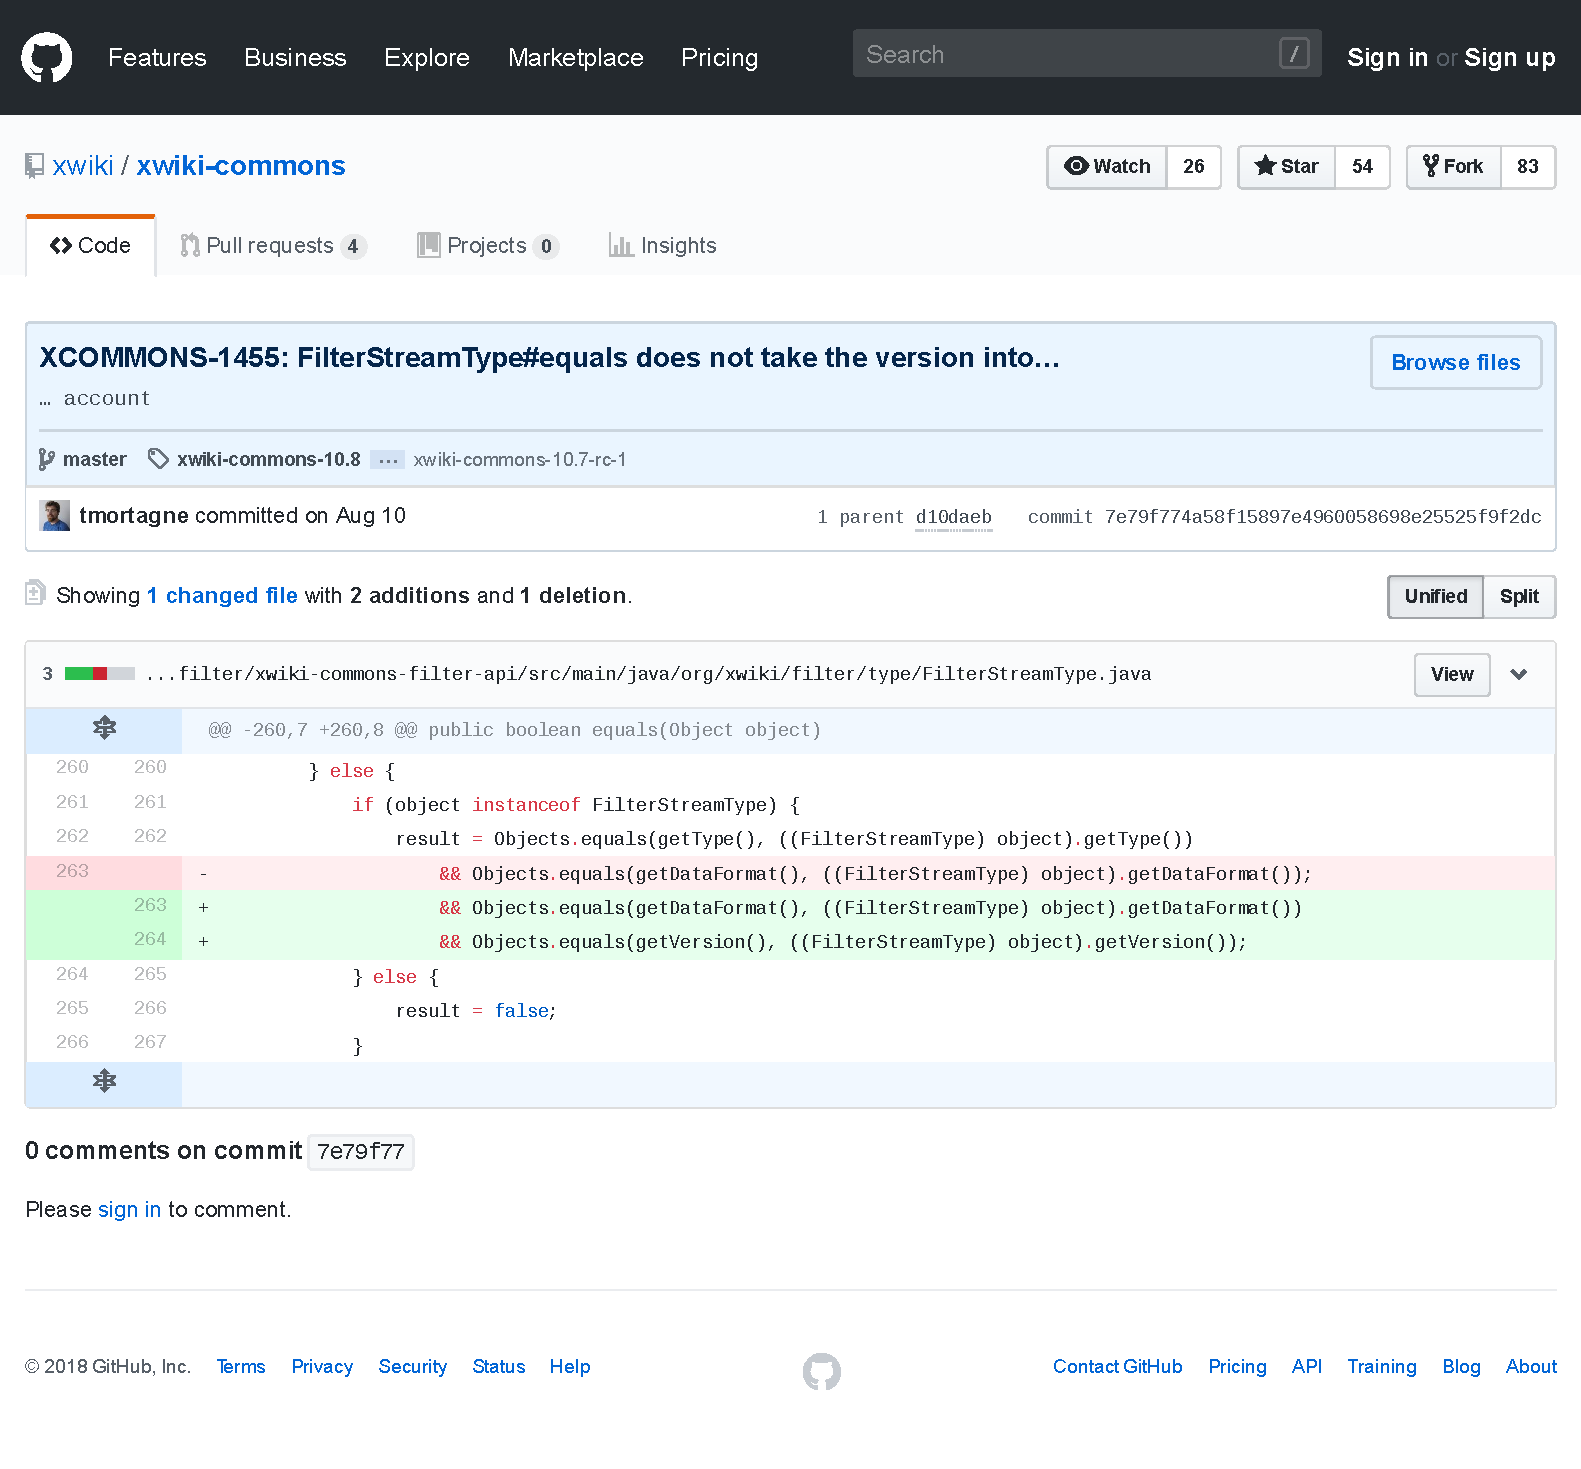
\includegraphics[width=.95\linewidth, trim=7.3cm 8.6cm 4.4cm 14.5cm, clip]{img/motivating_example.pdf}}
	\caption{Commit 7e79f77 on XWiki-Commons that changes the behavior without a test.}
	\label{fig:motivating_example}
\end{figure}

In this commit, the intent is to take into account the \texttt{version} (from method \texttt{getVersion}) in the \texttt{equals} method.
This change impacts the behavior of all methods that use it, \texttt{equals} being a highly used method.
Such a central behavioral change may impact the whole program, and the lack of a test case for this new behavior may have dramatic consequences in the future.
Without a test case, this change could be reverted and go undetected by the test suite and the Continuous Integration server, \ie the build would still pass.
Yet, a user of this program would encounter new errors, because of the changed behavior.
The developer took a risk when committing this change without a test case.

This extension of \dspot in continuous integration aims at mitigating such risk: 
test amplification aims at ensuring that every commit include a new test method or a modification of an existing test method.
In this chapter, I study \dspot's ability to automatically obtain a test method that highlights the behavioral change introduced by a commit.
This test method allows to identify the behavioral difference between the two versions of the program. 
The goal is to use this new test method to ensure that any changed behavior can be caught in the future.

What I propose is as follows: 
when Continuous Integration is triggered, 
rather than just executing the test suite to find regressions, 
it could also run an analysis of the commit to know if it contains a behavioral change, 
in the form of a new method or the modification of an existing one.
If there is no appropriate test method to detect a behavioral change, the approach would provide one. 
DCI would take as input the commit and a test suite, and generate a new test method that detects the behavioral change.

\subsection{Practibility}
\label{subsec:dci:background:praticability}

Following, a description of a complete scenario to sum up the vision of the approach's usage.

A developer commits a change into the program.
The Continuous Integration service is triggered;
the CI analyzes the commit.
There are two potential outcomes:
1) the developer provided a new test method or a modification to an existing one. 
In this case, the CI runs as usual, \eg it executes the test suite;
2) the developer did not provide a new test nor the modification of an existing one, the CI runs DCI on the commit to obtain a test method that detects the behavioral change and present it to the developer.
The developer can then validate the new test method that detects the behavioral change.
Following the test selection\autoref{subsec:dci:introduction:goal}, the new test method passes on the pre-commit version but fails on the post-commit version.
The current amplified test method cannot be added to the test suite, since it fails.
However, this test method is still useful, since one has only to negate the failing assertions, \eg change an \texttt{assertTrue} into an \texttt{assertFalse}, to obtain a valid and passing test method that explicitly executes the new behavior.
This can be done manually or automatically with approaches such as ReAssert\cite{ReAssert}.

\TODO{is this okay ? the definition of DSPOT says that dspot runs well on unit test}
From my experience, unit tests (vs integration test) are the best target for DCI
The reasons are behind the very nature of unit tests:
First, they have a small scope, which allow DCI to intensify its search while an integration test, that contains a lot of code, would make DCI explore the neighborhood in different ways.
Second, that is a consequence of the first, the unit tests are fast to be executed against integration test.
Since DCI needs to execute 5 times the tests under amplification, it means that DCI would be executed faster when it amplifies unit tests than when it amplified integration tests.

DCI has been designed to be easy to use.
The only cost of DCI is the time to set it up: in the ideal, happy-path case, it is meant to be a single command line through Maven goals.
Once DCI is set up in continuous integration, it automatically runs at each commit and developers directly benefit from amplified test methods that strengthen the existing test suite.

%
%   Behavioral Change
%
\subsection{Behavioral Change}
\label{subsec:dci:background:behavioral-change}

A \emph{behavioral change} is a source-code modification that triggers a new state for some inputs \cite{saff2004experimental}.
Considering the pre-commit version $P$ and the post-commit version $P'$ of a program, the commit introduces a behavioral change if it is possible to implement a test case that can trigger and observe the change, \ie, it passes on $P$ and fails on $P'$, or the opposite.
In short, the behavioral change must have an impact on the observable behavior of the program.

%
%   Behavioral Change Detection
%
\subsection{Behavioral Change Detection}
\label{subsec:dci:background:behavioral-change-detection}

Behavioral change detection is the task of identifying or generating a test or an input that distinguishes a behavioral change between two versions of the same program.
In this chapter, I propose a novel approach to detect behavioral changes based on test amplification.

% -----------------------
%  CONTRIBUTIONS
% -----------------------

\section{Behavioral Change Detection Approach}
\label{sec:dci:techniques}

\subsection{Overview of DCI}
\label{sec:dci:techniques:overview}

DCI takes as input a program, its test suite, and a commit modifying the program.
The commit, as done in version control systems, is basically the diff between two consecutive versions of the program.
%
% output
DCI outputs new test methods that detect the behavioral difference between the pre- and post-commit versions of the program.
The new tests pass on a given version, but fail on the other, demonstrating the presence of a behavioral change captured.% by an assertion.

DCI computes the code coverage of the diff and selects test methods accordingly. % to this diff coverage.
Then it applies \dspot to amplify and generation generate new test methods that detect the behavioral change.

\autoref{fig:global_approach} sums up the different phases of the approach:
1) Compute the diff coverage and select the tests to be amplified;
2) Amplify the selected tests based on the pre-commit version;
3) Execute amplified test methods against the post-commit version, and keep the failing test methods.
This process produces test methods that pass on the pre-commit version, fail on the post-commit version, hence they detect at least one behavioral change introduced by a given commit.

\begin{figure}
    \fbox{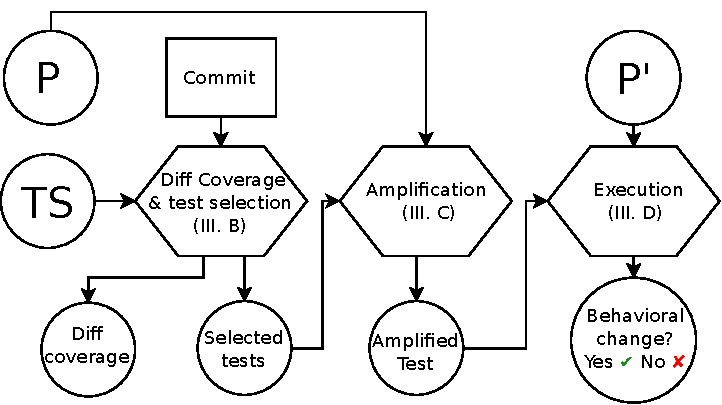
\includegraphics[width=.95\linewidth]{img/global_flow.pdf}}
    \caption{Overview of the approach to detect behavioral changes in commits.}
    \label{fig:global_approach}
\end{figure}

\subsection{Test Selection and Diff Coverage}
\label{subsec:compute_diff_coverage}
DCI implements a feature that:
\begin{enumerate*}
\item reports the diff coverage of a commit, and
\item selects the set of unit tests that execute the diff.
\end{enumerate*}
%
To do so, DCI first computes the code coverage for the whole test suite.
Second, it identifies the test methods that hit the statements modified by the diff. 
Third, it produces the two outcomes elicited earlier: the diff coverage, computed as the ratio of statements in the diff covered by the test suite over the total number of statements in the diff and the list of test methods that cover the diff.
%
Then, it selects only test methods that are present in pre-commit version (\ie, it ignores the test methods added in the commit, if any).
The final list of test methods that cover the diff is then used to seed the amplification process.

\subsection{Test Amplification}
\label{sec:dci:techniques:amplification}

Once DCI have the initial tests that cover the diff, DCI amplifies them using DSpot.

\subsection{Execution and Change Detection}
\label{sec:dci:techniques:execution-change-detection}

The final step performed by DCI consists in checking whether that the amplified test methods detect behavioral changes.
Because DCI amplifies test methods using the pre-commit version, all amplified test methods pass on this version, by construction. 
Consequently, for the last step, DCI runs the amplified test methods only on the post-commit version. 
Every test that fails is in fact detecting a behavioral change introduced by the commit, and is a success. DCI keeps the tests that successfully detect behavioral changes.

\subsection{Implementation}
\label{sec:dci:techniques:implementation}

DCI is implemented in Java and is built on top of the OpenClover and Gumtree~\cite{falleri:hal-01054552} libraries.
It computes the global coverage of the test suite with OpenClover, which instruments and executes the test suite.
Then, it uses Gumtree to have an AST representation of the diff.
DCI matches the diff with the test that executes those lines. 
Through its Maven plugin, DCI can be seamlessly implemented into continuous integration.
DCI is publicly available on \gh.\footnote{\url{https://github.com/STAMP-project/dspot.git}}

\section{Evaluation}
\label{sec:dci:evaluation}

To evaluate the DCI approach, we design an experimental protocol to answer the following research questions:

\newcommand{\rqcharacteristics}{\RQ{1}{What are the characteristics of commits with behavioral changes in the context of continuous integration?}}
\newcommand{\rqdetection}{\RQ{1}{To what extent are DCI$_{AAMPL}$ and DCI$_{SBAMPL}$ able to produce amplified test methods that detect the behavioral changes?}}
\newcommand{\rqselection}{\RQ{3}{What is the effectiveness of our test selection method?}}
\newcommand{\rqhuman}{\RQ{4}{How do human and generated tests that detect behavioral changes differ?}}
\newcommand{\rqiteration}{\RQ{2}{What  is the impact of the number of iteration performed by  DCI$_{SBAMPL}$?}}

\noindent
\begin{itemize}
% \item \rqcharacteristics
\item \rqdetection
\item \rqiteration
\item \rqselection
\item \rqhuman
\end{itemize}

\subsection{Benchmark}
\label{sec:benchmark}
To the best of our knowledge, there is no benchmark of commits in Java with behavioral changes in the literature. Consequently, we devise a project and commit selection procedure in order to construct a benchmark for our approach.

\paragraph{Project selection}
We need software projects that are
1) publicly-available,
2) written in Java,
3) and use continuous integration.
%
We pick the projects from the dataset in \cite{descartes} and \cite{dspot-emse}, which is composed of mature Java projects from \gh.

\paragraph{Commit selection}
%To select commits, we apply the following procedure.
We take commits in inverse chronological order, from newest to oldest.
%this result in commits buildable and analyzable with the current version of build and test tools;
We select the first ten commits that match the following criteria:
1) the commit modifies Java files (most behavioral changes are source code changes.\footnote{We are aware that behavioral changes can be introduced in other ways, such as modifying dependencies or configuration files \cite{Test:Coverage:Evolution}.});
% ground-truth
2) the commit provides or modifies a manually written test that detects a behavioral change. 
To verify this property, we execute the test on the pre-commit version. 
If it fails, it means that the test detects at least 1 behavioral change.
We will use this test as a \textit{ground-truth test} in \textbf{RQ4}.
3) The changes of the commit must be covered by the pre-commit test suite.
To do so, we compute the diff coverage. 
If the coverage is 0\%, we discard the commit. 
We do this because if the change is not covered, we cannot select any test methods to be amplified, which is what we want to evaluate.

Together, these criteria ensure that all selected commits:
1) introduce behavioral changes,
2) provide or modify a manually written test case that detects a behavioral change (which will be used as ground-truth for comparing generated tests), and
3) that there is at least 1 test in the pre-commit version of the program that executes the diff and can be used to seed the amplification process.
4) There is no structural change in the commit between both versions, \eg no change in method signature and deletion of classes (this is ensured since the pre-commit test suite compiles and runs against the post-commit version of the program and vice-versa.)

\paragraph{Final benchmark}
\begin{table}[h]
\centering
\def\arraystretch{1}
\setlength\tabcolsep{0.8pt}
\caption{Considered Period for Selecting Commits.}
\begin{tabular}{lc|rr|cccc}
\hline
project &
LOC &
\begin{tabular}{c}start\\date\end{tabular}&
\begin{tabular}{c}end\\date\end{tabular}&
\begin{tabular}{c}\#total\\commits\end{tabular}&
\begin{tabular}{c}\#discarded\\commits\end{tabular}&
\begin{tabular}{c}\#matching\\commits\end{tabular}&
\begin{tabular}{c}\#selected\\commits\end{tabular}\\
\hline
\scriptsize{commons-io}	&	59607	&	9/10/2015	&	9/29/2018	&	385	&	375	&	16(4.16\%)	&	10	\\
\rowcolor[HTML]{EFEFEF}
\scriptsize{commons-lang}	&	77410	&	11/22/2017	&	10/9/2018	&	227	&	217	&	13(5.73\%)	&	10	\\
\scriptsize{gson}	&	49766	&	6/14/2016	&	10/9/2018	&	159	&	149	&	13(8.18\%)	&	10	\\
\rowcolor[HTML]{EFEFEF}
\scriptsize{jsoup}	&	20088	&	12/21/2017	&	10/10/2018	&	50	&	40	&	11(22.00\%)	&	10	\\
\scriptsize{mustache.java}	&	10289	&	7/6/2016	&	04/18/2019	&	68	&	58	&	11(16.18\%)	&	10	\\
\rowcolor[HTML]{EFEFEF}
\scriptsize{xwiki-commons}	&	87289	&	10/31/2017	&	9/29/2018	&	687	&	677	&	23(3.35\%)	&	10	\\
\end{tabular}
\label{tab:benchmark}
\end{table}

\autoref{tab:benchmark} shows the main statistics on the benchmark dataset. % construction.
The first column is the name of the considered project;
The second column is the date at which we did the analysis;
The third column is the date of the oldest commit for the project;
The fourth, fifth, sixth and seventh are respectively the total number of commit we analyze, the total number of commits we discard, the number of commits that match all our criteria but the third (there is no test in the pre-commit that execute the change and the number of commit we select).
We note that our benchmark is only composed of recent commits from notable open-source projects and is available on \gh at \url{https://github.com/STAMP-project/dspot-experiments}.

\subsection{Protocol}
\label{subsec:protocol}

To answer \textbf{RQ1}, we run DCI$_{AAMPL}$ and DCI$_{SBAMPL}$ on the benchmark projects.
We then report the total number of behavioral changes successfully detected by DCI, \ie the number of commits for which DCI generates at least 1 test method that passes on the pre-commit version but fails on the post-commit version.
We also discuss 1 case study of a successful behavioral change detection.

To answer \textbf{RQ2}, we run DCI$_{SBAMPL}$ for 1, 2 and 3 iterations on the benchmark projects.
We report the number of behavioral changes successfully detected for each number of iterations in the main loop.
We report also the number amplified test methods that detect the behavioral changes for each commit for 10 different seeds to study the impact of the randomness on the output of DSpot
We perform a Kruskal-Wallis test statistic on these numbers.

The null hypothesis is the following: The population median of all of the groups are equal

The alternative hypothesis is: at least one population median of one group is different from the population median of at least one other group

We take a confidence level of 95\%, or $\alpha = 0.05$.

For \textbf{RQ3}, the test selection method is considered effective if the tests selected to be amplified semantically relate to the code changed by the commit. 
To assess this, we perform a manual analysis.% as follows.
We randomly select 1 commit per project in the benchmark, and we manually analyze whether the automatically selected tests for this commit are semantically related to the behavioral changes in the commit. 
%This research question aims at validating the test selection according to a diff of DCI.

To answer \textbf{RQ4}, we use the ground-truth tests written or modified by developers in the selected commits. % written by the humans.
We manually compare the amplified test methods that detect behavioral changes to the human tests, for 1 commit per project.
%For this, we take only consider commits for which DCI has been able to produce at least one test method that detects the behavioral change. 

\subsection{Results}
\label{subsec:result}
\begin{table}
\centering
\small
\def\arraystretch{0.3}%  1 is the default, change whatever you need
\setlength\tabcolsep{.35pt} % default value: 6pt
\caption{Performance evaluation of DCI on 60 commits from 6 large open-source projects.}
%\rotvertical{
\label{tab:overall_result}
\begin{tabular}{l|c|rcccc|c|cc|cc|cc|cc}
&
id&
date&
\#Test&
\begin{tabular}{c}\#Modified\\Tests\end{tabular}&
{\color{ForestGreen}{+\xspace}} / {\color{red}{-\xspace}}&
Cov&
\begin{tabular}{c}\#Selected\\Tests\end{tabular}&
\begin{tabular}{c}\#\aampl\\Tests\end{tabular}&
Time&
\begin{tabular}{c}\#\sbampl\\Tests\end{tabular}&
Time\\\\
\hline
\multirow{11}{*}{\rotvertical{commons-io}}
&  c6b8a38  &  6/12/18 &  1348  &  2  &  {\color{ForestGreen}{104\xspace}} / {\color{red}{3\xspace}}  &  100.0  &  3  &  0  &  10.0s  &  0  &  98.0s\\
&  2736b6f  &  12/21/17 &  1343  &  2  &  {\color{ForestGreen}{164\xspace}} / {\color{red}{1\xspace}}  &  1.79  &  8  &  0  &  19.0s  &  \cmark(12)  &  76.3m\\
&  a4705cc  &  4/29/18 &  1328  &  1  &  {\color{ForestGreen}{37\xspace}} / {\color{red}{0\xspace}}  &  100.0  &  2  &  0  &  10.0s  &  0  &  38.1m\\
&  f00d97a  &  5/2/17 &  1316  &  10  &  {\color{ForestGreen}{244\xspace}} / {\color{red}{25\xspace}}  &  100.0  &  2  &  \cmark(1)  &  10.0s  &  \cmark(39)  &  27.0s\\
&  3378280  &  4/25/17 &  1309  &  2  &  {\color{ForestGreen}{5\xspace}} / {\color{red}{5\xspace}}  &  100.0  &  1  &  \cmark(1)  &  9.0s  &  \cmark(11)  &  24.0s\\
&  703228a  &  12/2/16 &  1309  &  1  &  {\color{ForestGreen}{6\xspace}} / {\color{red}{0\xspace}}  &  50.0  &  8  &  0  &  19.0s  &  0  &  71.0m\\
&  a7bd568  &  9/24/16 &  1163  &  1  &  {\color{ForestGreen}{91\xspace}} / {\color{red}{83\xspace}}  &  50.0  &  8  &  0  &  20.0s  &  0  &  65.2m\\
&  81210eb  &  6/2/16 &  1160  &  1  &  {\color{ForestGreen}{10\xspace}} / {\color{red}{2\xspace}}  &  100.0  &  1  &  0  &  8.0s  &  \cmark(8)  &  23.0s\\
&  57f493a  &  11/19/15 &  1153  &  1  &  {\color{ForestGreen}{15\xspace}} / {\color{red}{1\xspace}}  &  100.0  &  8  &  0  &  7.0s  &  0  &  54.0s\\
&  5d072ef  &  9/10/15 &  1125  &  12  &  {\color{ForestGreen}{74\xspace}} / {\color{red}{34\xspace}}  &  68.42  &  25  &  \cmark(6)  &  29.0s  &  \cmark(1538)  &  2.2h\\
\hline
\rowcolor[HTML]{EFEFEF}
&  total  &  \xspace{} &  \xspace{}  &  \xspace{}  &  \xspace{}  &  \xspace{}  &  66  &  0.80  &  avg(14.5s)  &  160.80  &  avg(38.8m)\\
\hline
\multirow{11}{*}{\rotvertical{commons-lang}}
&  f56931c  &  7/2/18 &  4105  &  1  &  {\color{ForestGreen}{30\xspace}} / {\color{red}{4\xspace}}  &  25.0  &  42  &  0  &  2.4m  &  0  &  8.6h\\
&  87937b2  &  5/22/18 &  4101  &  1  &  {\color{ForestGreen}{114\xspace}} / {\color{red}{0\xspace}}  &  77.78  &  16  &  0  &  35.0s  &  0  &  18.1m\\
&  09ef69c  &  5/18/18 &  4100  &  1  &  {\color{ForestGreen}{10\xspace}} / {\color{red}{1\xspace}}  &  100.0  &  4  &  0  &  16.0s  &  0  &  98.8m\\
&  3fadfdd  &  5/10/18 &  4089  &  1  &  {\color{ForestGreen}{7\xspace}} / {\color{red}{1\xspace}}  &  100.0  &  9  &  0  &  17.0s  &  \cmark(4)  &  17.2m\\
&  e7d16c2  &  5/9/18 &  4088  &  1  &  {\color{ForestGreen}{13\xspace}} / {\color{red}{1\xspace}}  &  33.33  &  7  &  0  &  16.0s  &  \cmark(2)  &  15.1m\\
&  50ce8c4  &  3/8/18 &  4084  &  4  &  {\color{ForestGreen}{40\xspace}} / {\color{red}{1\xspace}}  &  90.91  &  2  &  \cmark(1)  &  28.0s  &  \cmark(135)  &  2.0m\\
&  2e9f3a8  &  2/11/18 &  4084  &  2  &  {\color{ForestGreen}{79\xspace}} / {\color{red}{4\xspace}}  &  30.0  &  47  &  0  &  79.0s  &  0  &  66.5m\\
&  c8e61af  &  2/10/18 &  4082  &  1  &  {\color{ForestGreen}{8\xspace}} / {\color{red}{1\xspace}}  &  100.0  &  10  &  0  &  17.0s  &  0  &  16.0s\\
&  d8ec011  &  11/12/17 &  4074  &  1  &  {\color{ForestGreen}{11\xspace}} / {\color{red}{1\xspace}}  &  100.0  &  5  &  0  &  31.0s  &  0  &  2.3m\\
&  7d061e3  &  11/22/17 &  4073  &  1  &  {\color{ForestGreen}{16\xspace}} / {\color{red}{1\xspace}}  &  100.0  &  8  &  0  &  17.0s  &  0  &  11.4m\\
\hline
\rowcolor[HTML]{EFEFEF}
&  total  &  \xspace{} &  \xspace{}  &  \xspace{}  &  \xspace{}  &  \xspace{}  &  150  &  0.10  &  avg(40.5s)  &  14.10  &  avg(74.7m)\\
\hline
\multirow{11}{*}{\rotvertical{gson}}
&  b1fb9ca  &  9/22/17 &  1035  &  1  &  {\color{ForestGreen}{23\xspace}} / {\color{red}{0\xspace}}  &  50.0  &  166  &  0  &  4.2m  &  0  &  92.5m\\
&  7a9fd59  &  9/18/17 &  1033  &  2  &  {\color{ForestGreen}{21\xspace}} / {\color{red}{2\xspace}}  &  83.33  &  14  &  0  &  15.0s  &  \cmark(108)  &  2.1m\\
&  03a72e7  &  8/1/17 &  1031  &  2  &  {\color{ForestGreen}{43\xspace}} / {\color{red}{11\xspace}}  &  68.75  &  371  &  0  &  7.7m  &  0  &  3.2h\\
&  74e3711  &  6/20/17 &  1029  &  1  &  {\color{ForestGreen}{68\xspace}} / {\color{red}{5\xspace}}  &  8.0  &  1  &  0  &  4.0s  &  0  &  16.0s\\
&  ada597e  &  5/31/17 &  1029  &  2  &  {\color{ForestGreen}{28\xspace}} / {\color{red}{3\xspace}}  &  100.0  &  5  &  0  &  8.0s  &  0  &  8.7m\\
&  a300148  &  5/31/17 &  1027  &  7  &  {\color{ForestGreen}{103\xspace}} / {\color{red}{2\xspace}}  &  18.18  &  665  &  0  &  9.2m  &  \cmark(6)  &  4.9h\\
&  9a24219  &  4/19/17 &  1019  &  1  &  {\color{ForestGreen}{13\xspace}} / {\color{red}{1\xspace}}  &  100.0  &  36  &  0  &  2.2m  &  0  &  48.9m\\
&  9e6f2ba  &  2/16/17 &  1018  &  2  &  {\color{ForestGreen}{56\xspace}} / {\color{red}{2\xspace}}  &  50.0  &  9  &  0  &  32.0s  &  \cmark(2)  &  8.5m\\
&  44cad04  &  11/26/16 &  1015  &  1  &  {\color{ForestGreen}{6\xspace}} / {\color{red}{0\xspace}}  &  100.0  &  2  &  0  &  15.0s  &  \cmark(37)  &  40.0s\\
&  b2c00a3  &  6/14/16 &  1012  &  4  &  {\color{ForestGreen}{242\xspace}} / {\color{red}{29\xspace}}  &  60.71  &  383  &  0  &  7.9m  &  0  &  3.6h\\
\hline
\rowcolor[HTML]{EFEFEF}
&  total  &  \xspace{} &  \xspace{}  &  \xspace{}  &  \xspace{}  &  \xspace{}  &  1652  &  0.00  &  avg(3.2m)  &  15.30  &  avg(86.5m)\\
\hline
\multirow{11}{*}{\rotvertical{jsoup}}
&  426ffe7  &  5/11/18 &  668  &  4  &  {\color{ForestGreen}{27\xspace}} / {\color{red}{46\xspace}}  &  64.71  &  27  &  \cmark(2)  &  42.0s  &  \cmark(198)  &  33.6m\\
&  a810d2e  &  4/29/18 &  666  &  1  &  {\color{ForestGreen}{27\xspace}} / {\color{red}{1\xspace}}  &  80.0  &  5  &  0  &  10.0s  &  0  &  26.6m\\
&  6be19a6  &  4/29/18 &  664  &  1  &  {\color{ForestGreen}{23\xspace}} / {\color{red}{1\xspace}}  &  50.0  &  50  &  0  &  69.0s  &  0  &  67.7m\\
&  e38dfd4  &  4/28/18 &  659  &  1  &  {\color{ForestGreen}{66\xspace}} / {\color{red}{15\xspace}}  &  90.0  &  18  &  0  &  35.0s  &  0  &  12.5m\\
&  e9feec9  &  4/15/18 &  654  &  1  &  {\color{ForestGreen}{15\xspace}} / {\color{red}{3\xspace}}  &  100.0  &  4  &  0  &  9.0s  &  0  &  95.0s\\
&  0f7e0cc  &  4/14/18 &  653  &  2  &  {\color{ForestGreen}{56\xspace}} / {\color{red}{15\xspace}}  &  84.62  &  330  &  0  &  6.5m  &  \cmark(36)  &  11.8h\\
&  2c4e79b  &  4/14/18 &  650  &  2  &  {\color{ForestGreen}{82\xspace}} / {\color{red}{2\xspace}}  &  50.0  &  44  &  0  &  67.0s  &  0  &  4.7h\\
&  e5210d1  &  12/22/17 &  647  &  1  &  {\color{ForestGreen}{3\xspace}} / {\color{red}{3\xspace}}  &  100.0  &  14  &  0  &  9.0s  &  0  &  4.9m\\
&  df272b7  &  12/22/17 &  647  &  2  &  {\color{ForestGreen}{17\xspace}} / {\color{red}{1\xspace}}  &  100.0  &  13  &  0  &  9.0s  &  0  &  4.6m\\
&  3676b13  &  12/21/17 &  648  &  6  &  {\color{ForestGreen}{104\xspace}} / {\color{red}{12\xspace}}  &  38.46  &  239  &  0  &  6.2m  &  \cmark(52)  &  6.8h\\
\hline
\rowcolor[HTML]{EFEFEF}
&  total  &  \xspace{} &  \xspace{}  &  \xspace{}  &  \xspace{}  &  \xspace{}  &  744  &  0.20  &  avg(101.0s)  &  28.60  &  avg(2.6h)\\
\hline
\multirow{11}{*}{\rotvertical{mustache.java}}
&  a1197f7  &  1/25/18 &  228  &  1  &  {\color{ForestGreen}{43\xspace}} / {\color{red}{57\xspace}}  &  77.78  &  131  &  0  &  11.8m  &  \cmark(204)  &  10.1h\\
&  8877027  &  11/19/17 &  227  &  1  &  {\color{ForestGreen}{22\xspace}} / {\color{red}{2\xspace}}  &  33.33  &  47  &  0  &  7.3m  &  0  &  100.2m\\
&  d8936b4  &  2/1/17 &  219  &  2  &  {\color{ForestGreen}{46\xspace}} / {\color{red}{6\xspace}}  &  60.0  &  168  &  0  &  12.7m  &  0  &  84.2m\\
&  88718bc  &  1/25/17 &  216  &  2  &  {\color{ForestGreen}{29\xspace}} / {\color{red}{1\xspace}}  &  100.0  &  1  &  \cmark(1)  &  7.0s  &  \cmark(149)  &  3.7m\\
&  339161f  &  9/23/16 &  214  &  2  &  {\color{ForestGreen}{32\xspace}} / {\color{red}{10\xspace}}  &  77.78  &  123  &  0  &  8.6m  &  \cmark(1312)  &  5.8h\\
&  774ae7a  &  8/10/16 &  214  &  2  &  {\color{ForestGreen}{17\xspace}} / {\color{red}{2\xspace}}  &  100.0  &  11  &  0  &  66.0s  &  \cmark(124)  &  6.8m\\
&  94847cc  &  7/29/16 &  214  &  2  &  {\color{ForestGreen}{17\xspace}} / {\color{red}{2\xspace}}  &  100.0  &  95  &  0  &  11.5m  &  \cmark(2509)  &  21.4h\\
&  eca08ca  &  7/14/16 &  212  &  4  &  {\color{ForestGreen}{47\xspace}} / {\color{red}{10\xspace}}  &  80.0  &  18  &  0  &  87.0s  &  0  &  41.8m\\
&  6d7225c  &  7/7/16 &  212  &  2  &  {\color{ForestGreen}{42\xspace}} / {\color{red}{4\xspace}}  &  80.0  &  18  &  0  &  87.0s  &  0  &  40.1m\\
&  8ac71b7  &  7/6/16 &  210  &  10  &  {\color{ForestGreen}{167\xspace}} / {\color{red}{31\xspace}}  &  40.0  &  20  &  0  &  2.1m  &  \cmark(124)  &  5.6m\\
\hline
\rowcolor[HTML]{EFEFEF}
&  total  &  \xspace{} &  \xspace{}  &  \xspace{}  &  \xspace{}  &  \xspace{}  &  632  &  0.10  &  avg(5.8m)  &  442.20  &  avg(4.2h)\\
\hline
\multirow{11}{*}{\rotvertical{xwiki-commons}}
&  ffc3997  &  7/27/18 &  1081  &  0  &  {\color{ForestGreen}{125\xspace}} / {\color{red}{18\xspace}}  &  21.05  &  1  &  0  &  29.0s  &  0  &  18.0s\\
&  ced2635  &  8/13/18 &  1081  &  1  &  {\color{ForestGreen}{21\xspace}} / {\color{red}{14\xspace}}  &  60.0  &  5  &  0  &  93.0s  &  0  &  2.5h\\
&  10841b1  &  8/1/18 &  1061  &  1  &  {\color{ForestGreen}{107\xspace}} / {\color{red}{19\xspace}}  &  30.0  &  51  &  0  &  5.7m  &  0  &  3.4h\\
&  848c984  &  7/6/18 &  1074  &  1  &  {\color{ForestGreen}{154\xspace}} / {\color{red}{111\xspace}}  &  17.65  &  1  &  0  &  28.0s  &  0  &  18.0s\\
&  adfefec  &  6/27/18 &  1073  &  1  &  {\color{ForestGreen}{17\xspace}} / {\color{red}{14\xspace}}  &  40.0  &  22  &  \cmark(1)  &  76.0s  &  \cmark(3)  &  14.9m\\
&  d3101ae  &  1/18/18 &  1062  &  2  &  {\color{ForestGreen}{71\xspace}} / {\color{red}{9\xspace}}  &  20.0  &  4  &  \cmark(1)  &  72.0s  &  \cmark(31)  &  41.4m\\
&  a0e8b77  &  1/18/18 &  1062  &  2  &  {\color{ForestGreen}{51\xspace}} / {\color{red}{8\xspace}}  &  42.86  &  4  &  \cmark(1)  &  72.0s  &  \cmark(60)  &  42.1m\\
&  78ff099  &  12/19/17 &  1061  &  1  &  {\color{ForestGreen}{16\xspace}} / {\color{red}{0\xspace}}  &  33.33  &  2  &  0  &  68.0s  &  \cmark(4)  &  6.6m\\
&  1b79714  &  11/13/17 &  1060  &  1  &  {\color{ForestGreen}{20\xspace}} / {\color{red}{5\xspace}}  &  60.0  &  22  &  0  &  78.0s  &  0  &  17.9m\\
&  6dc9059  &  10/31/17 &  1060  &  1  &  {\color{ForestGreen}{4\xspace}} / {\color{red}{14\xspace}}  &  88.89  &  22  &  0  &  79.0s  &  0  &  20.5m\\
\hline
\rowcolor[HTML]{EFEFEF}
&  total  &  \xspace{} &  \xspace{}  &  \xspace{}  &  \xspace{}  &  \xspace{}  &  134  &  0.30  &  avg(94.3s)  &  9.80  &  avg(49.5m)\\
\hline
\hline
&  total  &  \xspace{} &  \xspace{}  &  \xspace{}  &  \xspace{}  &  \xspace{}  &  3378  &  9(15)  &  avg(2.2m)  &  28(6708)  &  avg(109.4m)\\
\hline
\end{tabular}
%}
\end{table}

The overall results are reported in \autoref{tab:overall_result}.
The first column is the shortened commit id;
the second column is the commit date;
the third column column is the total number of test methods executed when building that version of the project;
the fourth and fifth columns are respectively the number of tests modified or added by the commit, and the size of the diff in terms of line additions (in green) and deletions (in red);
the sixth and seventh columns are respectively the diff coverage and the number of tests DCI selected;
the eighth column provides the amplification results for DCI$_{AAMPL}$, and it is either a \cmark with the number of amplified tests that detect a behavioral change or a \textit{-} if DCI did not succeed in generating a test that detects a change;
the ninth column displays the time spent on the amplification phase;
The tenth and the eleventh are respectively a \cmark with the number of amplified tests for DCI$_{SBAMPL}$  (or - if a change is not detected) for 3 iterations.

\subsubsection{Characteristics of commits with behavioral changes in the context of continuous integration}
\label{subsubsec:answerq1}

%We consider the first columns (under \textbf{RQ1} meta column) of \autoref{tab:overall_result}, which describe the characteristics of our novel benchmark.
%The columns under the \textbf{RQ1} meta column
In  this section, we describe the the characteristics of commits introducing behavioral changes in the context of continuous integration
The first five columns in \autoref{tab:overall_result} describe the characteristics of our benchmark.
% date
The commit dates show that the benchmark is only composed of recent commits.
The most recent is \textsc{gson\#b1fb9ca}, authored 9/22/18, and the oldest is \textsc{commons-io\#5d072ef}, authored 9/10/15.
% now the number of tests
The number of test methods at the time of the commit shows two aspects of our benchmark:
1) we only have strongly tested projects;
2) we see that the number of tests evolve over time
%, witnessing the presence of 
due to test evolution.
%The fourth column shows that 
Every commit in the benchmark comes with test modifications (new tests or updated tests), and commit sizes are quite diverse.
%For instance, the first commit c6b8a38 has two modified tests.
%The fifth column shows the size of the commit diff in terms of added and removed lines.
%Overall, our selection criteria include a diversity of commit sizes. 
The three smallest commits are \textsc{commons-io\#703228a}, \textsc{gson\#44cad04} and \textsc{jsoup\#e5210d1} with 6 modifications, and the largest is \textsc{Gson\#45511fd} with 334 modifications.
%
Finally, 
%we consider the sixth column which gives the code coverage of the diff itself. 
on average, commits have 66.11\% coverage. 
The distribution of diff coverage is reported graphically by \autoref{fig:histdiffcoverage}: 
in commons-io all selected commits have more than 75\% coverage.
In XWiki-Commons, only 50\% of commits have more than 75\% coverage. Overall, 31 / 60 commits have at least 75\% of the changed lines covered.
This validates the correct implementation of our selection criteria that ensures the presence of a test specifying the behavioral change.

\begin{figure}
\centering
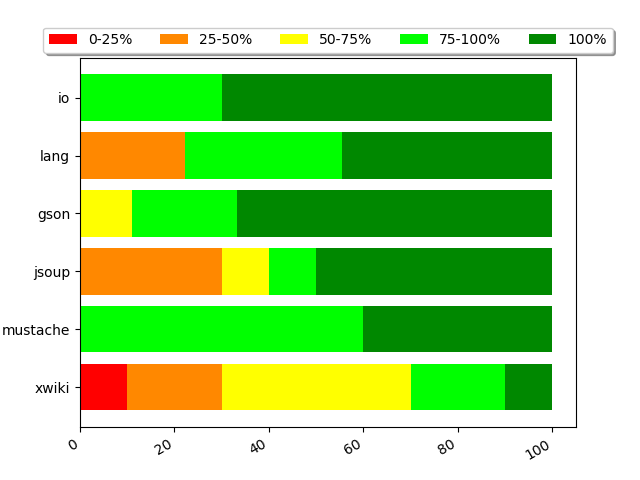
\includegraphics[width=.95\linewidth]{img/diff_cov_hist.png}
\caption{Distribution of diff coverage per project of our benchmark.}
\label{fig:histdiffcoverage}
\end{figure}

% recap of RQ1.
Thanks to our selection criteria, we have a curated benchmark of 50 commits with a behavioral change, coming from notable open-source projects, and covering a diversity of commit sizes. The benchmark is publicly available and documented for future research on this topic.

%%%%%%%%%%%%%%%%%%%%%%%%%%%%%%%%%%%%%%%%%%%%%%%%%%%%%
%%%%%%%%%%%%%%%%%%%%%%%%%%%%%%%%%%%%%%%%%%%%%%%%%%%%%
%% RESULTS RQ2
%%%%%%%%%%%%%%%%%%%%%%%%%%%%%%%%%%%%%%%%%%%%%%%%%%%%%
%%%%%%%%%%%%%%%%%%%%%%%%%%%%%%%%%%%%%%%%%%%%%%%%%%%%%
\subsubsection{\rqdetection}
\label{subsubsec:answerq2}

We now focus on the last 4 columns of \autoref{tab:overall_result}.
For instance, for \textsc{commons-io\#f00d97a} (4$^{th}$ row), DCI$_{AAMPL}$ generated 39 amplified tests that detect the behavioral change. 
For \textsc{commons-io\#81210eb} (8$^{th}$ row), only the \sbampl version of DCI detects the change.
%
Overall, using only \aampl, DCI generates amplified tests that detect 9 out of 60 behavioral changes.
Meanwhile, using \sbampl only, DCI generates amplified tests that detect 28 out of 60 behavioral changes.

Regarding the number of generated tests.
\DCII generates a large number of test cases, compared to \DCIA only (15 versus 6708, see column ``total'' at the bottom of the table). 
Both \DCIA and \DCIA can generate amplified tests, however since \DCIA does not produce a large amount of test methods the developers do not have to triage a large set of test cases. 
Also, since \DCIA only adds assertions, the amplified tests are easier to understand than the ones generated by \DCII.

% time
\DCII takes more time than \DCIA (for successful cases 38.7 seconds versus 3.3 hours on average).
The difference comes from the time consumed during the exploration of the input space in the case of \DCII, while \DCIA focuses on the amplification of assertions only, which represents a much smaller space of solutions. 

Overall, DCI successfully generates amplified tests that detect a behavioral change in 46\% of the commits in our benchmark(28 out of 60).
Recall that the 60 commits that we analyze are real changes that fix bugs in complex code bases.
They represent modifications, sometimes deep in the code, that represent challenges with respect to testability~\cite{voas1995software}.
Consequently, the fact DCI can generate test cases that detect behavioral changes, is considered an achievement.
The commits for which DCI fails to detect the change can be considered as a target for future research on this topic.

Now, we manually analyze a successful case where DCI detects the behavioral change.
We select commit \textsc{3fadfdd}\footnote{\url{https://github.com/apache/commons-lang/commit/3fadfdd}} from commons-lang, which is succinct enough to be discussed in the paper.
The diff is shown in \autoref{fig:diff_commons_lang_success}.

\begin{figure}[h]
\centering
\fbox{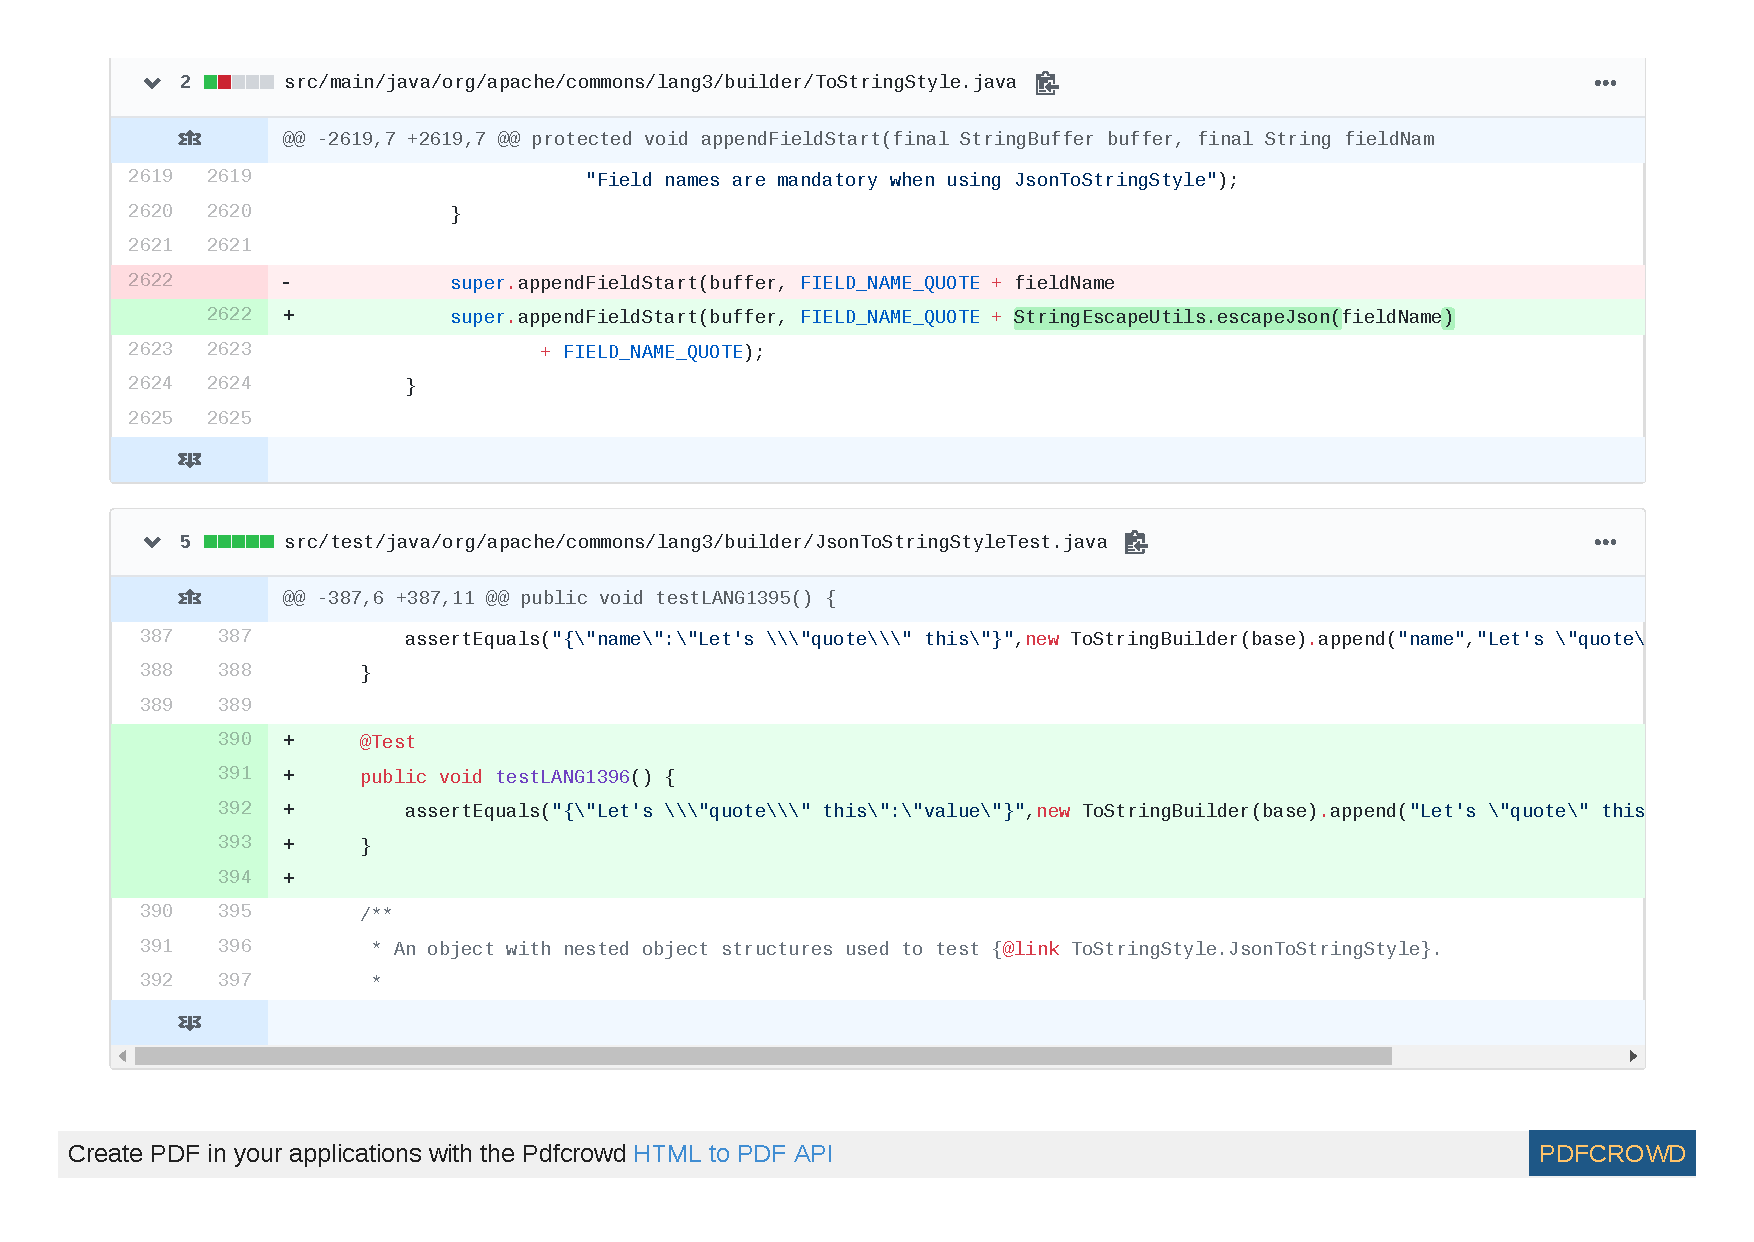
\includegraphics[width=.95\linewidth, trim=4.5cm 14.85cm 6.5cm 4.3cm, clip]{img/diff/success-diff-commons-lang.pdf}}
\caption{Diff of commit \textsc{3fadfdd} from commons-lang.}
\label{fig:diff_commons_lang_success}
\end{figure}

The developer added a method call to a method that escapes specials characters in a string. 
The changes come with a new test method that specifies the new behavior. 

DCI starts the amplification from the \texttt{testNestingPerson} test method defined in \texttt{JsonToStringStyleTest}. The test is selected for amplification because it triggers the execution of the changed line.

\begin{figure}[h]
\centering
\fbox{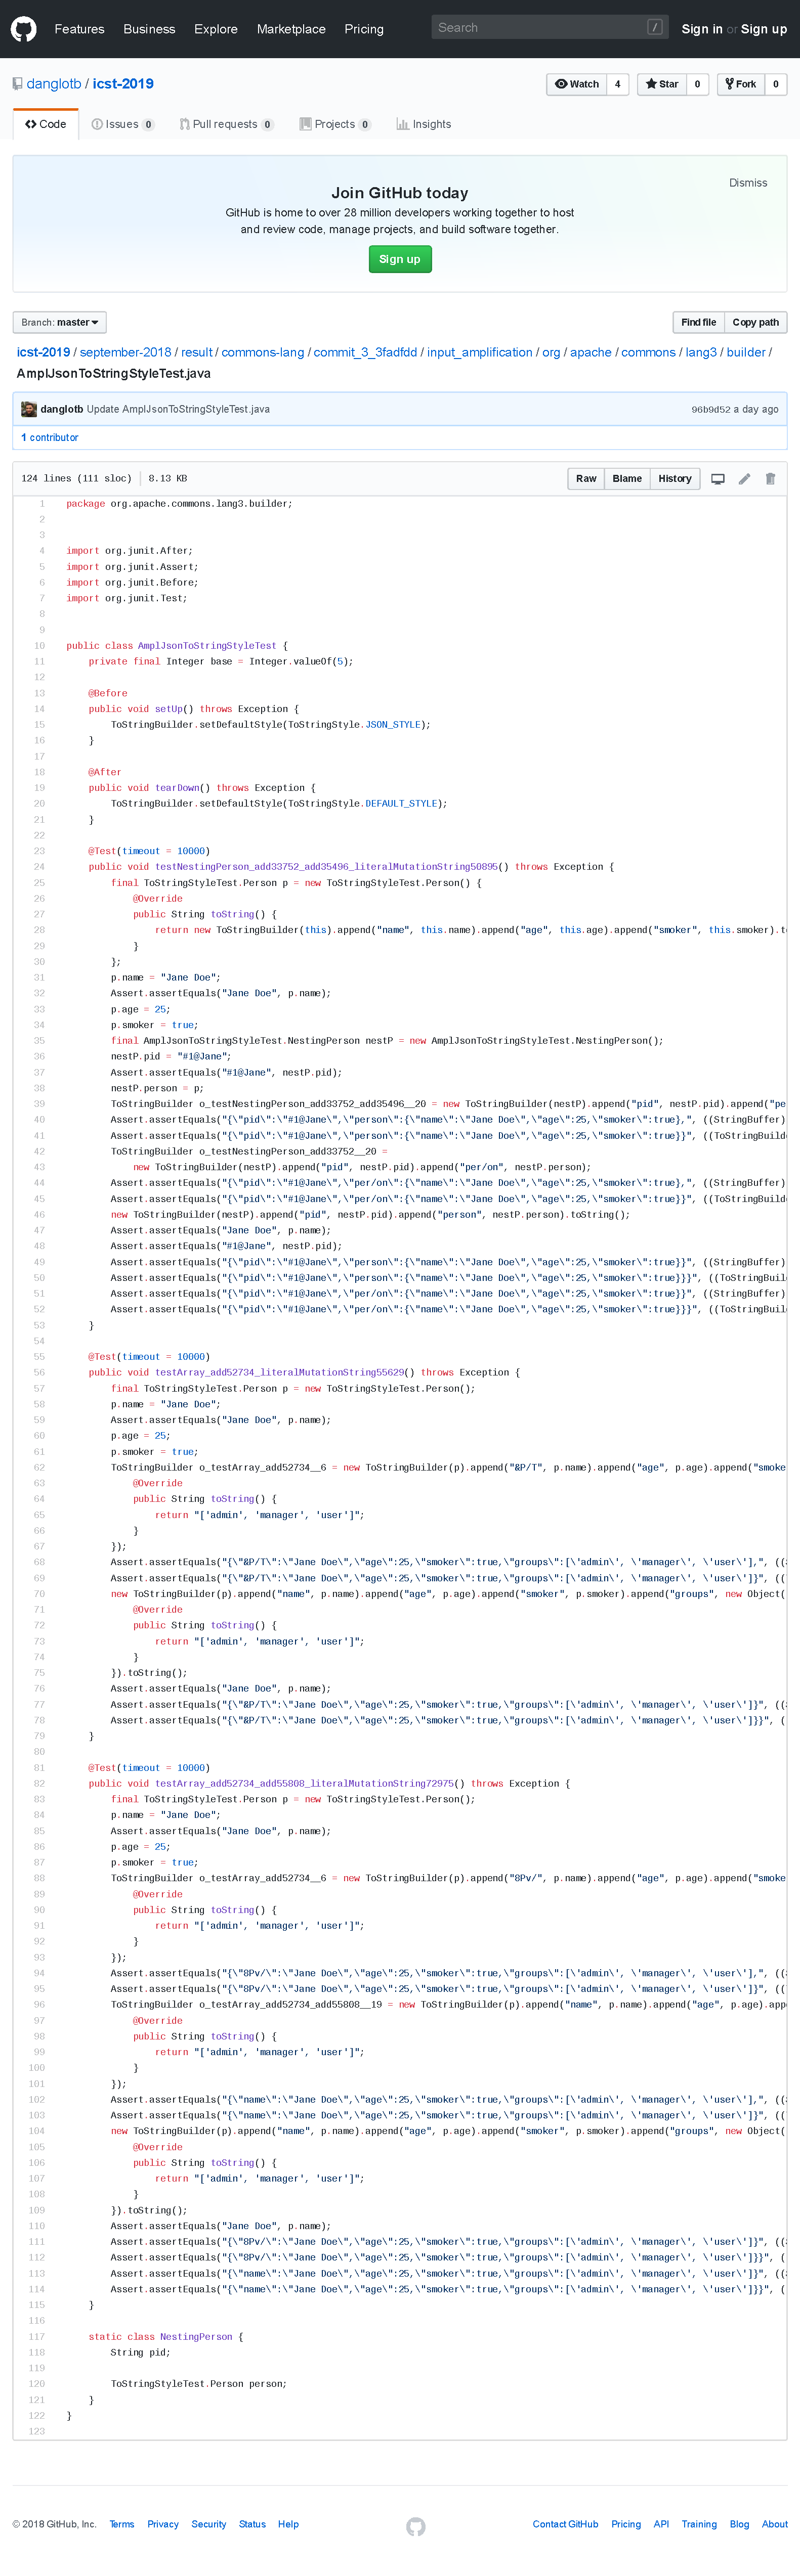
\includegraphics[width=.95\linewidth, trim=3.7cm 46.5cm 9.65cm 38.3cm, clip]{img/amplified/success-ampl-commons-lang.pdf}}
\caption{Test generated by DCI that detects the behavioral change of \textsc{3fadfdd} from commons-lang.}
\label{fig:amplified_commons_lang_success}
\end{figure}

We show in \autoref{fig:amplified_commons_lang_success} 
the resulting amplified test method.
From this test method, DCI generates an amplified test method shown in \autoref{fig:amplified_commons_lang_success}. 
In this generated test, \sbampl applies 2 input transformations: 1 duplication of method call and 1 character replacement in an existing String literal.
The latter transformation is the key transformation: DCI replaced an 's' inside "person" by '/' resulting in "per/on" where "/" is a special character that must be escaped (Line 2). 
Then, DCI generated 11 assertions, based on the modified inputs. 
The amplified test the behavioral change:
in the pre-commit version, the expected value is: \texttt{"\{ ... per/on":\{"name":"Jane Doe" ...\}"} while in the post-commit version it is \texttt{"\{ ... per\textbackslash/on":\{"name":"Jane Doe" ...\}"} (Line 3).
 
%recap RQ2
\begin{mdframed}
Answer to \textbf{RQ1}: Overall, DCI is capable of detecting the behavioral changes in a total of 28/60 commits. Individually, \DCII finds changes in 28/60, while \DCIA in 9/60 commits.
Since \DCII also uses \aampl to generate assertions, all \DCIA's commits are contained in \DCII's. However, the search-based algorithm, through exploration, finds many more behavioral changes, making it more effective albeit at the cost of execution time.
\end{mdframed}

%%%%%%%%%%%%%%%%%%%%%%%%%%%%%%%%%%%%%%%%%%%%%%%%%%%%%
%%%%%%%%%%%%%%%%%%%%%%%%%%%%%%%%%%%%%%%%%%%%%%%%%%%%%
%% RESULTS RQ2 : ITERATION
%%%%%%%%%%%%%%%%%%%%%%%%%%%%%%%%%%%%%%%%%%%%%%%%%%%%%
%%%%%%%%%%%%%%%%%%%%%%%%%%%%%%%%%%%%%%%%%%%%%%%%%%%%%

\subsubsection{\rqiteration}
\label{subsubsec:answerqiteration}

The results are reported in \autoref{tab:overall_result_iteration}
This table can be read as follow:
the first column is the name of the project;
the second column is the commit identifier;
then, the third, fourth, fifth, sixth, seventh and eighth provide the amplification results and execution time for each number of iteration 1, 2, and 3. A \cmark indicates with the number of amplified tests that detect a behavioral change and a \textit{-} denotes that DCI did not succeed in generating a test that detects a change.

% number of detection
Overall, \DCII generates amplified tests that detect 21, 23, and 24 out of 60 behavioral changes for respectively $iteration=1$, $iteration=2$ and $iteration=3$.
The more iteration \DCII does, the more it explores, the more it generates amplified tests that detect the behavioral changes but the more it takes time also.
% difference in number of behavioral changes we detect
When \DCII is used with $iteration=3$, it generates amplified test methods that detect 3 more behavioral changes than when it is used with $iteration=1$ and 1 then when it is used with $iteration=2$. It represents an increase of 14\% and 4\% for respectively $iteration=1$ and $iteration=2$.

% number of test generated
In average, \DCII generates 18, 53, and 116 amplified tests for respectively $iteration=1$, $iteration=2$ and $iteration=3$. 
This number increases by 544\% from $iteration=1$ to $iteration=3$.
This increase is explained by the fact that \DCII explores more with more iteration and thus is able to generate more amplified test methods that detect the behavioral changes.

% time
In average \DCII takes 23, 64, and 105 minutes to perform the amplification for respectively $iteration=1$, $iteration=2$ and $iteration=3$.
This number increases by 356\% from $iteration=1$ to $iteration=3$.

\begin{table*}
\small
\def\arraystretch{1}%  1 is the default, change whatever you need
\setlength\tabcolsep{6pt} % default value: 6pt
\caption{Evaluation of the impact of the number of iteration done by \DCII on 60 commits from 6 open-source projects.}
%\rotvertical{
\label{tab:overall_result_iteration}
\begin{tabular}{l|c|cc|cc|cc}
&
id&
$it=1$&
Time&
$it=2$&
Time&
$it=3$&
Time\\
\midrule
\multirow{11}{*}{\rotverticalinv{commons-io}}
&  c6b8a38  &  0 &  25.0s  &  0  &  62.0s  &  0  &  98.0s\\
&  2736b6f  &  \cmark(1) &  26.1m  &  \cmark(2)  &  44.2m  &  \cmark(12)  &  76.3m\\
&  a4705cc  &  0 &  4.1m  &  0  &  21.1m  &  0  &  38.1m\\
&  f00d97a  &  \cmark(7) &  13.0s  &  \cmark(28)  &  19.0s  &  \cmark(39)  &  27.0s\\
&  3378280  &  \cmark(6) &  15.0s  &  \cmark(10)  &  20.0s  &  \cmark(11)  &  24.0s\\
&  703228a  &  0 &  30.3m  &  0  &  55.1m  &  0  &  71.0m\\
&  a7bd568  &  0 &  28.6m  &  0  &  52.0m  &  0  &  65.2m\\
&  81210eb  &  \cmark(2) &  14.0s  &  \cmark(4)  &  18.0s  &  \cmark(8)  &  23.0s\\
&  57f493a  &  0 &  20.0s  &  0  &  32.0s  &  0  &  54.0s\\
&  5d072ef  &  \cmark(461) &  32.2m  &  \cmark(1014)  &  65.5m  &  \cmark(1538)  &  2.2h\\
\midrule
\rowcolor[HTML]{EFEFEF}
&  total  &  477 &  2.0h  &  1058  &  4.0h  &  1608  &  6.5h\\
\midrule
&  average  &  47.70 &  12.3m  &  105.80  &  24.0m  &  160.80  &  38.8m\\
\midrule
\multirow{11}{*}{\rotverticalinv{commons-lang}}
&  f56931c  &  0 &  0.0s  &  0  &  3.7m  &  0  &  8.5m\\
&  87937b2  &  0 &  3.5m  &  0  &  10.5m  &  0  &  18.1m\\
&  09ef69c  &  0 &  97.0s  &  0  &  21.0m  &  0  &  98.8m\\
&  3fadfdd  &  \cmark(1) &  2.0m  &  \cmark(1)  &  9.3m  &  \cmark(4)  &  17.2m\\
&  e7d16c2  &  \cmark(3) &  111.0s  &  \cmark(2)  &  8.4m  &  \cmark(2)  &  15.1m\\
&  50ce8c4  &  \cmark(61) &  38.0s  &  \cmark(97)  &  78.0s  &  \cmark(135)  &  2.0m\\
&  2e9f3a8  &  0 &  11.4m  &  0  &  35.0m  &  0  &  66.5m\\
&  c8e61af  &  0 &  16.0s  &  0  &  16.0s  &  0  &  16.0s\\
&  d8ec011  &  0 &  36.0s  &  0  &  68.0s  &  0  &  2.3m\\
&  7d061e3  &  0 &  79.0s  &  0  &  5.8m  &  0  &  11.4m\\
\midrule
\rowcolor[HTML]{EFEFEF}
&  total  &  65 &  23.3m  &  100  &  96.4m  &  141  &  4.0h\\
\midrule
&  average  &  6.50 &  2.3m  &  10.00  &  9.6m  &  14.10  &  24.0m\\
\midrule
\multirow{11}{*}{\rotverticalinv{gson}}
&  b1fb9ca  &  0 &  14.6m  &  0  &  51.0m  &  0  &  92.5m\\
&  7a9fd59  &  \cmark(7) &  33.0s  &  \cmark(48)  &  73.0s  &  \cmark(108)  &  2.1m\\
&  03a72e7  &  0 &  30.2m  &  0  &  102.3m  &  0  &  3.2h\\
&  74e3711  &  0 &  6.0s  &  0  &  11.0s  &  0  &  16.0s\\
&  ada597e  &  0 &  61.0s  &  0  &  4.9m  &  0  &  8.7m\\
&  a300148  &  0 &  45.2m  &  \cmark(4)  &  2.6h  &  \cmark(6)  &  4.9h\\
&  9a24219  &  0 &  10.8m  &  0  &  28.4m  &  0  &  48.9m\\
&  9e6f2ba  &  0 &  79.0s  &  0  &  4.5m  &  \cmark(2)  &  8.5m\\
&  44cad04  &  \cmark(4) &  21.0s  &  \cmark(21)  &  30.0s  &  \cmark(37)  &  40.0s\\
&  b2c00a3  &  0 &  31.5m  &  0  &  111.8m  &  0  &  3.6h\\
\midrule
\rowcolor[HTML]{EFEFEF}
&  total  &  11 &  2.3h  &  73  &  7.7h  &  153  &  14.4h\\
\midrule
&  average  &  1.10 &  13.6m  &  7.30  &  46.0m  &  15.30  &  86.5m\\
\midrule
\multirow{11}{*}{\rotverticalinv{jsoup}}
&  426ffe7  &  \cmark(126) &  5.4m  &  \cmark(172)  &  19.2m  &  \cmark(198)  &  33.6m\\
&  a810d2e  &  0 &  90.0s  &  0  &  13.9m  &  0  &  26.6m\\
&  6be19a6  &  0 &  8.1m  &  0  &  39.7m  &  0  &  67.7m\\
&  e38dfd4  &  0 &  117.0s  &  0  &  6.3m  &  0  &  12.5m\\
&  e9feec9  &  0 &  20.0s  &  0  &  50.0s  &  0  &  95.0s\\
&  0f7e0cc  &  \cmark(1) &  2.4h  &  \cmark(7)  &  6.8h  &  \cmark(36)  &  11.8h\\
&  2c4e79b  &  0 &  7.1m  &  0  &  34.1m  &  0  &  4.7h\\
&  e5210d1  &  0 &  45.0s  &  0  &  2.3m  &  0  &  4.9m\\
&  df272b7  &  0 &  43.0s  &  0  &  2.2m  &  0  &  4.6m\\
&  3676b13  &  \cmark(6) &  21.4m  &  \cmark(35)  &  2.9h  &  \cmark(52)  &  6.8h\\
\midrule
\rowcolor[HTML]{EFEFEF}
&  total  &  133 &  3.2h  &  214  &  11.6h  &  286  &  25.8h\\
\midrule
&  average  &  13.30 &  19.4m  &  21.40  &  69.8m  &  28.60  &  2.6h\\
\midrule
\multirow{11}{*}{\rotverticalinv{mustache.java}}
&  a1197f7  &  \cmark(28) &  5.9h  &  \cmark(124)  &  8.4h  &  \cmark(204)  &  10.1h\\
&  8877027  &  0 &  30.5m  &  0  &  58.4m  &  0  &  100.2m\\
&  d8936b4  &  0 &  3.2m  &  0  &  4.8m  &  0  &  84.2m\\
&  88718bc  &  \cmark(13) &  78.0s  &  \cmark(85)  &  2.5m  &  \cmark(149)  &  3.7m\\
&  339161f  &  \cmark(143) &  115.9m  &  \cmark(699)  &  4.1h  &  \cmark(1312)  &  5.8h\\
&  774ae7a  &  \cmark(18) &  2.7m  &  \cmark(65)  &  4.7m  &  \cmark(124)  &  6.8m\\
&  94847cc  &  \cmark(122) &  5.3h  &  \cmark(580)  &  10.4h  &  \cmark(2509)  &  21.4h\\
&  eca08ca  &  0 &  8.1m  &  0  &  24.3m  &  0  &  41.8m\\
&  6d7225c  &  0 &  7.9m  &  0  &  26.8m  &  0  &  40.1m\\
&  8ac71b7  &  \cmark(2) &  2.7m  &  \cmark(48)  &  3.8m  &  \cmark(124)  &  5.6m\\
\midrule
\rowcolor[HTML]{EFEFEF}
&  total  &  326 &  14.0h  &  1601  &  25.0h  &  4422  &  42.0h\\
\midrule
&  average  &  32.60 &  84.3m  &  160.10  &  2.5h  &  442.20  &  4.2h\\
\midrule
\multirow{11}{*}{\rotverticalinv{xwiki-commons}}
&  ffc3997  &  0 &  19.0s  &  0  &  18.0s  &  0  &  18.0s\\
&  ced2635  &  0 &  8.0m  &  0  &  31.8m  &  0  &  2.5h\\
&  10841b1  &  0 &  56.2m  &  0  &  2.9h  &  0  &  3.4h\\
&  848c984  &  0 &  18.0s  &  0  &  17.0s  &  0  &  18.0s\\
&  adfefec  &  \cmark(22) &  3.5m  &  \cmark(57)  &  9.9m  &  \cmark(3)  &  14.9m\\
&  d3101ae  &  \cmark(9) &  11.6m  &  \cmark(12)  &  28.2m  &  \cmark(31)  &  41.4m\\
&  a0e8b77  &  \cmark(10) &  12.0m  &  \cmark(17)  &  28.2m  &  \cmark(60)  &  42.1m\\
&  78ff099  &  \cmark(4) &  2.6m  &  \cmark(4)  &  4.6m  &  \cmark(4)  &  6.6m\\
&  1b79714  &  0 &  4.0m  &  0  &  10.7m  &  0  &  17.9m\\
&  6dc9059  &  0 &  4.0m  &  0  &  10.8m  &  0  &  20.5m\\
\midrule
\rowcolor[HTML]{EFEFEF}
&  total  &  45 &  102.8m  &  90  &  4.9h  &  98  &  8.2h\\
\midrule
&  average  &  4.50 &  10.3m  &  9.00  &  29.7m  &  9.80  &  49.5m\\
\midrule
\midrule
&  total  &  23(1057) &  23.7h  &  24(3136)  &  54.9h  &  25(6708)  &  100.9h\\
\bottomrule
\end{tabular}
%}
\end{table*}

\paragraph{Impact of the randomness}

The number of amplified test methods obtained by the different seeds are reported in \autoref{tab:overall_result_seeds}.
The result of the Kruskal-Wallis test is:  p-value=0.96.
$p-value>\alpha$ which means that we keep the null hypothesis: 
The population median of all of the groups are equal.
This means that, in general, the choice of the seeds has not a significant impact of the overall result of DCI.

\begin{table*}
\small
\def\arraystretch{.5}%  1 is the default, change whatever you need
\setlength\tabcolsep{3pt} % default value: 6pt
\caption{Number of amplified test methods obtained by DCI for 10 different seeds. The first column is the id of the commit. The second column is the result obtained with the default seed, used during the evaluation for \rqdetection. The ten following columns are the result obtained for the 10 different seeds.}
\label{tab:overall_result_seeds}
\begin{tabular}{l|c|llllllllll}
&id&0&1&2&3&4&5&6&7&8&9\\
\hline
\multirow{11}{*}{\rotvertical{commons-io}}
 & c6b8a38 & - & - & - & - & - & - & - & - & - & -\\
 & 2736b6f & 1 & 1 & - & 2 & 1 & 1 & 2 & 1 & - & -\\
 & a4705cc & - & - & - & - & - & - & - & - & - & -\\
 & f00d97a & 7 & 7 & 7 & 7 & 7 & 7 & 7 & 7 & 7 & 7\\
 & 3378280 & 6 & 6 & 6 & 6 & 6 & 6 & 6 & 6 & 6 & 6\\
 & 703228a & - & - & - & - & - & 2 & - & 1 & - & -\\
 & a7bd568 & - & - & - & - & - & 2 & - & 1 & - & -\\
 & 81210eb & 2 & 2 & 2 & 2 & 2 & 2 & 2 & 2 & 2 & 2\\
 & 57f493a & - & - & - & - & - & - & - & - & - & -\\
 & 5d072ef & 464 & 462 & 463 & 463 & 461 & 462 & 465 & 460 & 463 & 462\\
\hline
\multirow{11}{*}{\rotvertical{commons-lang}}
 & f56931c & - & - & - & - & 1 & - & 1 & 1 & 1 & 1\\
 & 87937b2 & - & - & - & - & - & - & - & - & - & -\\
 & 09ef69c & - & - & - & - & - & - & - & - & - & -\\
 & 3fadfdd & 1 & - & 2 & 3 & 3 & 2 & 1 & - & - & 1\\
 & e7d16c2 & - & 1 & - & - & 1 & 1 & - & 1 & 1 & 1\\
 & 50ce8c4 & 61 & 63 & 62 & 57 & 58 & 60 & 61 & 62 & 63 & 61\\
 & 2e9f3a8 & - & - & - & - & - & - & - & - & - & -\\
 & c8e61af & - & - & - & - & - & - & - & - & - & -\\
 & d8ec011 & - & - & - & - & - & - & - & - & - & -\\
 & 7d061e3 & - & - & - & - & - & - & - & - & - & -\\
\hline
\multirow{11}{*}{\rotvertical{gson}}
 & b1fb9ca & - & - & - & - & - & - & - & - & - & -\\
 & 7a9fd59 & 7 & 7 & 7 & 7 & 7 & 7 & 7 & 7 & 7 & 7\\
 & 03a72e7 & - & - & - & - & - & - & - & - & 0 & 3\\
 & 74e3711 & - & - & - & - & - & - & - & - & - & -\\
 & ada597e & - & - & - & - & - & - & - & - & - & -\\
 & a300148 & - & - & - & - & - & - & - & - & - & -\\
 & 9a24219 & - & - & - & - & - & - & - & - & - & -\\
 & 9e6f2ba & - & - & - & - & - & - & - & - & - & -\\
 & 44cad04 & 5 & 4 & 6 & 4 & 4 & 4 & 4 & 4 & 3 & 5\\
 & b2c00a3 & - & - & - & - & - & - & - & - & - & -\\
\hline
\multirow{11}{*}{\rotvertical{jsoup}}
 & 426ffe7 & 125 & 125 & 123 & 126 & 126 & 127 & 123 & 121 & 119 & 121\\
 & a810d2e & - & - & - & - & - & - & - & - & - & -\\
 & 6be19a6 & - & - & - & - & - & - & - & - & - & -\\
 & e38dfd4 & - & - & - & - & - & - & - & - & - & -\\
 & e9feec9 & - & - & - & - & - & 1 & - & 1 & - & -\\
 & 0f7e0cc & - & - & 1 & 1 & - & 1 & 1 & - & 1 & -\\
 & 2c4e79b & - & - & - & - & - & - & - & - & - & -\\
 & e5210d1 & - & - & - & - & - & - & - & - & - & -\\
 & df272b7 & - & - & - & - & - & - & - & - & - & -\\
 & 3676b13 & 3 & 6 & 2 & 3 & 4 & 1 & 1 & 1 & 1 & -\\
\hline
\multirow{11}{*}{\rotvertical{mustache.java}}
 & a1197f7 & 22 & - & - & - & - & - & - & - & - & -\\
 & 8877027 & - & - & - & - & - & - & - & - & - & -\\
 & d8936b4 & - & - & - & - & - & - & - & - & - & -\\
 & 88718bc & 12 & 11 & 13 & 13 & 11 & 13 & 12 & 12 & 12 & 12\\
 & 339161f & 135 & 146 & - & - & - & - & 138 & - & - & 144\\
 & 774ae7a & 23 & 18 & 3 & 17 & 18 & 15 & 16 & 19 & 17 & 20\\
 & 94847cc & - & - & 112 & - & 61 & 72 & 57 & 40 & 42 & 37\\
 & eca08ca & - & - & - & - & - & - & - & - & - & -\\
 & 6d7225c & - & - & - & - & - & - & - & - & - & -\\
 & 8ac71b7 & 2 & 2 & 2 & 2 & 2 & 2 & 2 & 2 & 2 & 2\\
\hline
\multirow{11}{*}{\rotvertical{xwiki-commons}}
 & ffc3997 & - & - & - & - & - & - & - & - & - & -\\
 & ced2635 & - & - & - & - & - & - & - & - & - & -\\
 & 10841b1 & - & - & - & - & - & - & - & - & - & -\\
 & 848c984 & - & - & - & - & - & - & - & - & - & -\\
 & adfefec & 1 & 1 & 1 & 1 & 1 & 1 & 1 & 1 & 1 & 1\\
 & d3101ae & 18 & 15 & 13 & 14 & 15 & 14 & - & 15 & 12 & 15\\
 & a0e8b77 & 19 & - & 14 & 15 & 17 & 15 & 16 & 16 & 13 & 16\\
 & 78ff099 & 4 & 4 & 4 & 4 & 4 & 4 & 4 & 4 & 4 & 4\\
 & 1b79714 & - & - & - & - & - & - & - & - & - & -\\
 & 6dc9059 & - & - & - & - & - & - & - & - & - & -\\
\hline
\end{tabular}
\end{table*}

%recap RQ2
\begin{mdframed}
Answer to \textbf{RQ2}: \DCII detects  21, 23, and 24 behavioral changes out of 60 for respectively $iteration=1$, $iteration=2$ and $iteration=3$.
The number of iteration done by \DCII impacts the number of behavioral changes detected, the number of amplified test methods obtained and the execution time.
\end{mdframed}

%%%%%%%%%%%%%%%%%%%%%%%%%%%%%%%%%%%%%%%%%%%%%%%%%%%%%
%%%%%%%%%%%%%%%%%%%%%%%%%%%%%%%%%%%%%%%%%%%%%%%%%%%%%
%% RESULTS RQ3
%%%%%%%%%%%%%%%%%%%%%%%%%%%%%%%%%%%%%%%%%%%%%%%%%%%%%
%%%%%%%%%%%%%%%%%%%%%%%%%%%%%%%%%%%%%%%%%%%%%%%%%%%%%

\subsubsection{\rqselection}
\label{subsubsec:answerq3}

To answer \textbf{RQ3}, there is no quantitative approach to take, because there is no ground truth data or metrics to optimize. 
Per our protocol described in \autoref{subsec:protocol}, we answer this question based on manual analysis:
we randomly selected 1 commit per project, and we analyzed the relevance of the selected tests for amplification.

In order to give an intuition of what we consider as a relevant test selection for amplification, let us look at an example. 
If \texttt{TestX} is selected for amplification, following a change to method \texttt{X}, we consider this as relevant. The key is that DCI will generate an amplified test \texttt{TestX'} that is a variant of \texttt{TestX}, and, consequently, the developer will directly get the intention of the new test \texttt{TestX'} and what behavioral change it detects.

\textsc{Commons-io\#c6b8a38}\footnote{\url{https://github.com/apache/commons-io/commit/c6b8a38}}: our test selection returns 3 test methods: \texttt{testContentEquals}, \texttt{testCopyURLToFileWithTimeout} and \texttt{testCopyURLToFile} from the same test class: \texttt{FileUtilsTestCase}.
The considered commit modifies the method \texttt{copyToFile} from \texttt{FileUtils}. 
Two test methods out 3 (\texttt{testCopyURLToFileWithTimeout} and \texttt{testCopyURLToFile}) there is a link between the changed file and the intention of tests to be amplified. 
The selection is thus considered relevant.

\textsc{Commons-lang\#f56931c}\footnote{\url{https://github.com/apache/commons-lang/commit/f56931c}}: our test selection returns 39 test methods from 5 test classes: \texttt{FastDateFormat\_ParserTest}, \texttt{FastDateParserTest}, \texttt{DateUtilsTest}, \texttt{FastDateParser\_TimeZoneStrategyTest} and \texttt{FastDateParser\_MoreOrLessTest}.
This commit modifies the behavior of two methods: \texttt{simpleQuote} and \texttt{setCalendar} of class \texttt{FastDateParser}.
Our manual analysis reveals two intentions:
1) test behaviors related to parsing, 
1) test behaviors related to dates.
While this is meaningful, a set of 39 methods is clearly not a focused selection, not as focused as for the previous example.
It is considered as an half-success.

 \textsc{Gson\#9e6f2ba}\footnote{\url{https://github.com/google/gson/commit/9e6f2ba}}: our test selection returns 9 test methods from 5 different test classes.
 Three out of those five classes \texttt{JsonElementReaderTest}, \texttt{JsonReaderPathTest} and \texttt{JsonParserTest} relate to the class modified in the commit(\texttt{JsonTreeReader}).
The selection is thus considered relevant but unfocused.

 \textsc{Jsoup\#e9feec9}\footnote{\url{https://github.com/jhy/jsoup/commit/e9feec9}}, our test selection returns the 4 test methods defined in the \texttt{XmlTreeBuilderTest} class : \texttt{caseSensitiveDeclaration}, \texttt{handlesXmlDeclarationAsDeclaration}, \texttt{testDetectCharsetEncodingDeclaration} and \texttt{testParseDeclarationAttributes}.
 The commit modifies the behavior of the class \texttt{XmlTreeBuilder}.
Here, the test selection is relevant.
Actually, the ground-truth manual test added in the commit is also in the \texttt{XmlTreeBuilderTest} class.
If DCI proposes a new test there to capture the behavioral change, the developer will understand its relevance and its relation to the change.

\textsc{Mustache.java\#88718bc}\footnote{\url{https://github.com/spullara/mustache.java/commit/88718bc}}, our test selection returns the \texttt{testInvalidDelimiters} test method defined in the \texttt{com.github.mustachejava.InterpreterTest} test class.
The commit improves an error message when an invalid delimiter is used.
Here, the test selection is relevant since it selected \texttt{testInvalidDelimiters} which is the dedicated test to the usage of the test invalid delimiters.
This ground-truth test method is also in the test class \texttt{com.github.mustachejava.InterpreterTest}.

\textsc{Xwiki-commons\#848c984}\footnote{\url{https://github.com/xwiki/xwiki-commons/commit/848c984}} our test selection returns a single test method \texttt{createReference} from test class \texttt{XWikiDocumentTest}.
The main modification of this commit is on class \texttt{XWikiDocument}.
Since \texttt{XWikiDocumentTest} is the test class dedicated to \texttt{XWikiDocument}, this is considered as a success.

\begin{mdframed}
Answer to \textbf{RQ3}: 
In 4 out of 6 of the manually analyzed cases, the tests selected to be amplified relate, semantically, to the modified application code. 
In the 2 remaining cases, we selected over and above the tests to be amplified.
That is, we select tests whose intention is semantically pertinent to the change, but we also include tests that are not.
%the test intention is captured but not focused.
%, the test class name, method name and initialization code 
%This indicates that in the selected tests by DCI give the right context for the developer to understand what behavioral change is specified.
However, even in this case, DCI's test selection provides developers with important and targeted context to better understand the behavioral change at hand.
\end{mdframed}


%%%%%%%%%%%%%%%%%%%%%%%%%%%%%%%%%%%%%%%%%%%%%%%%%%%%%
%%%%%%%%%%%%%%%%%%%%%%%%%%%%%%%%%%%%%%%%%%%%%%%%%%%%%
%% RESULTS RQ4
%%%%%%%%%%%%%%%%%%%%%%%%%%%%%%%%%%%%%%%%%%%%%%%%%%%%%
%%%%%%%%%%%%%%%%%%%%%%%%%%%%%%%%%%%%%%%%%%%%%%%%%%%%%
\subsubsection{\rqhuman}
\label{subsubsec:answerq4}

When DCI generates an amplified test method that detects the behavioral change, we can compare it to the ground truth version (the test added in the commit) to see whether it captures the same behavioral change.
For each project, we select 1 successful application of DCI, and we compare the DCI test against the human test.
If they capture the same behavioral change, it means they have the same intention and we consider the amplification a success.

%%% COMMONS IO

\textsc{commons-io\#81210eb}\footnote{\url{https://github.com/apache/commons-io/commit/81210eb}}: This commit modifies the behavior of the \texttt{read()} method in \texttt{BoundedReader}.
\autoref{fig:ampl_commons-io} shows the test generated by \DCII.
This test is amplified from the existing \texttt{readMulti} test, which indicates that the intention is to test the read functionality.
The first line of the test is the construction of a \texttt{BoundedReader} object which is also the class modified by the commit.
\DCII modified the second parameter of the constructor call (transformed $3$ into a $0$) and generated two assertions (only 1 is shown).
The first assertion, associated to the new test input, captures the behavioral difference.
Overall, this can be considered as a successful amplication.

\begin{figure}[h]
\centering
\fbox{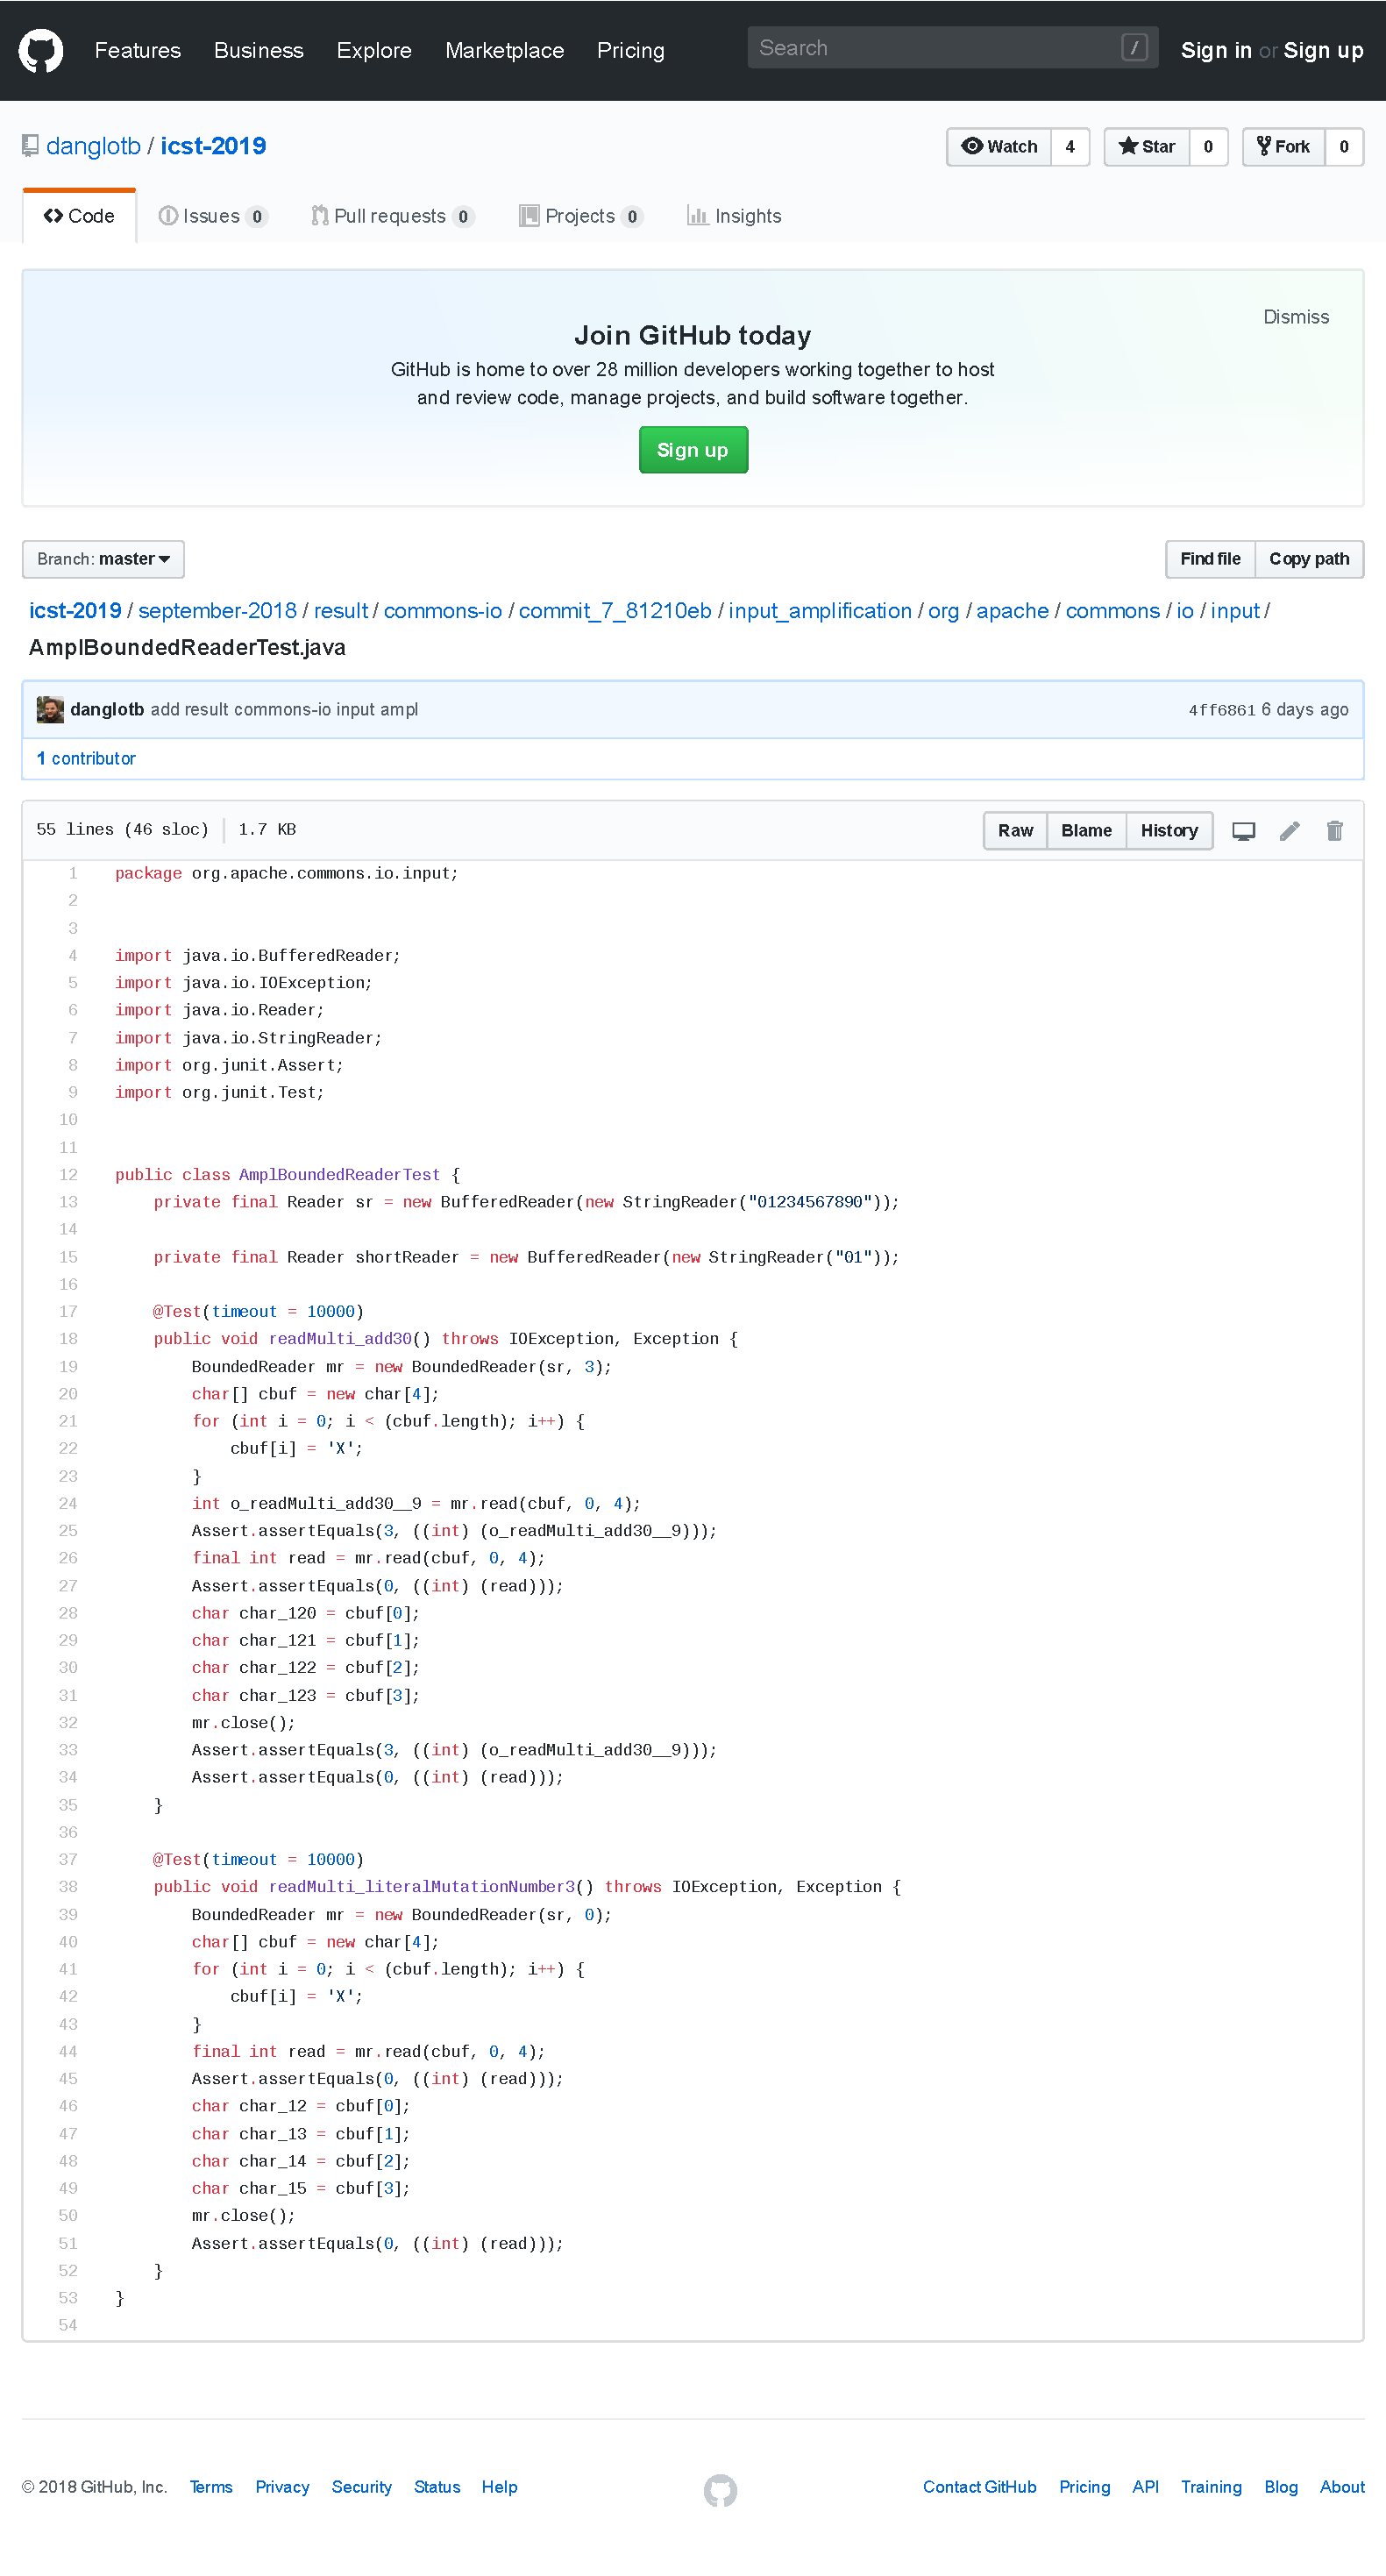
\includegraphics[width=.97\linewidth, trim=3.6cm 9.3cm 14.7cm 36.8cm, clip]{img/amplified/ampl-commons-io.pdf}}
\caption{Test generated by \DCII that detects the behavioral change introduced by commit \textsc{81210eb} in commons-io.}
\label{fig:ampl_commons-io}
\end{figure}

Now, let us look at the human test contained in the commit, shown in \autoref{fig:diff_commons-io}.
It captures the behavioral change with the timeout (the test timeouts on the pre-commit version and goes fast enough on the post-commit version). 
Furthermore, it only indirectly calls the changed method through a call to \texttt{readLine}.

In this case, the DCI test can be considered better than the developer test because
1) it relies on assertions and not on timeouts, and
2) it directly calls the changed method (\texttt{read}) instead of indirectly. 

\begin{figure}[h]
\centering
\fbox{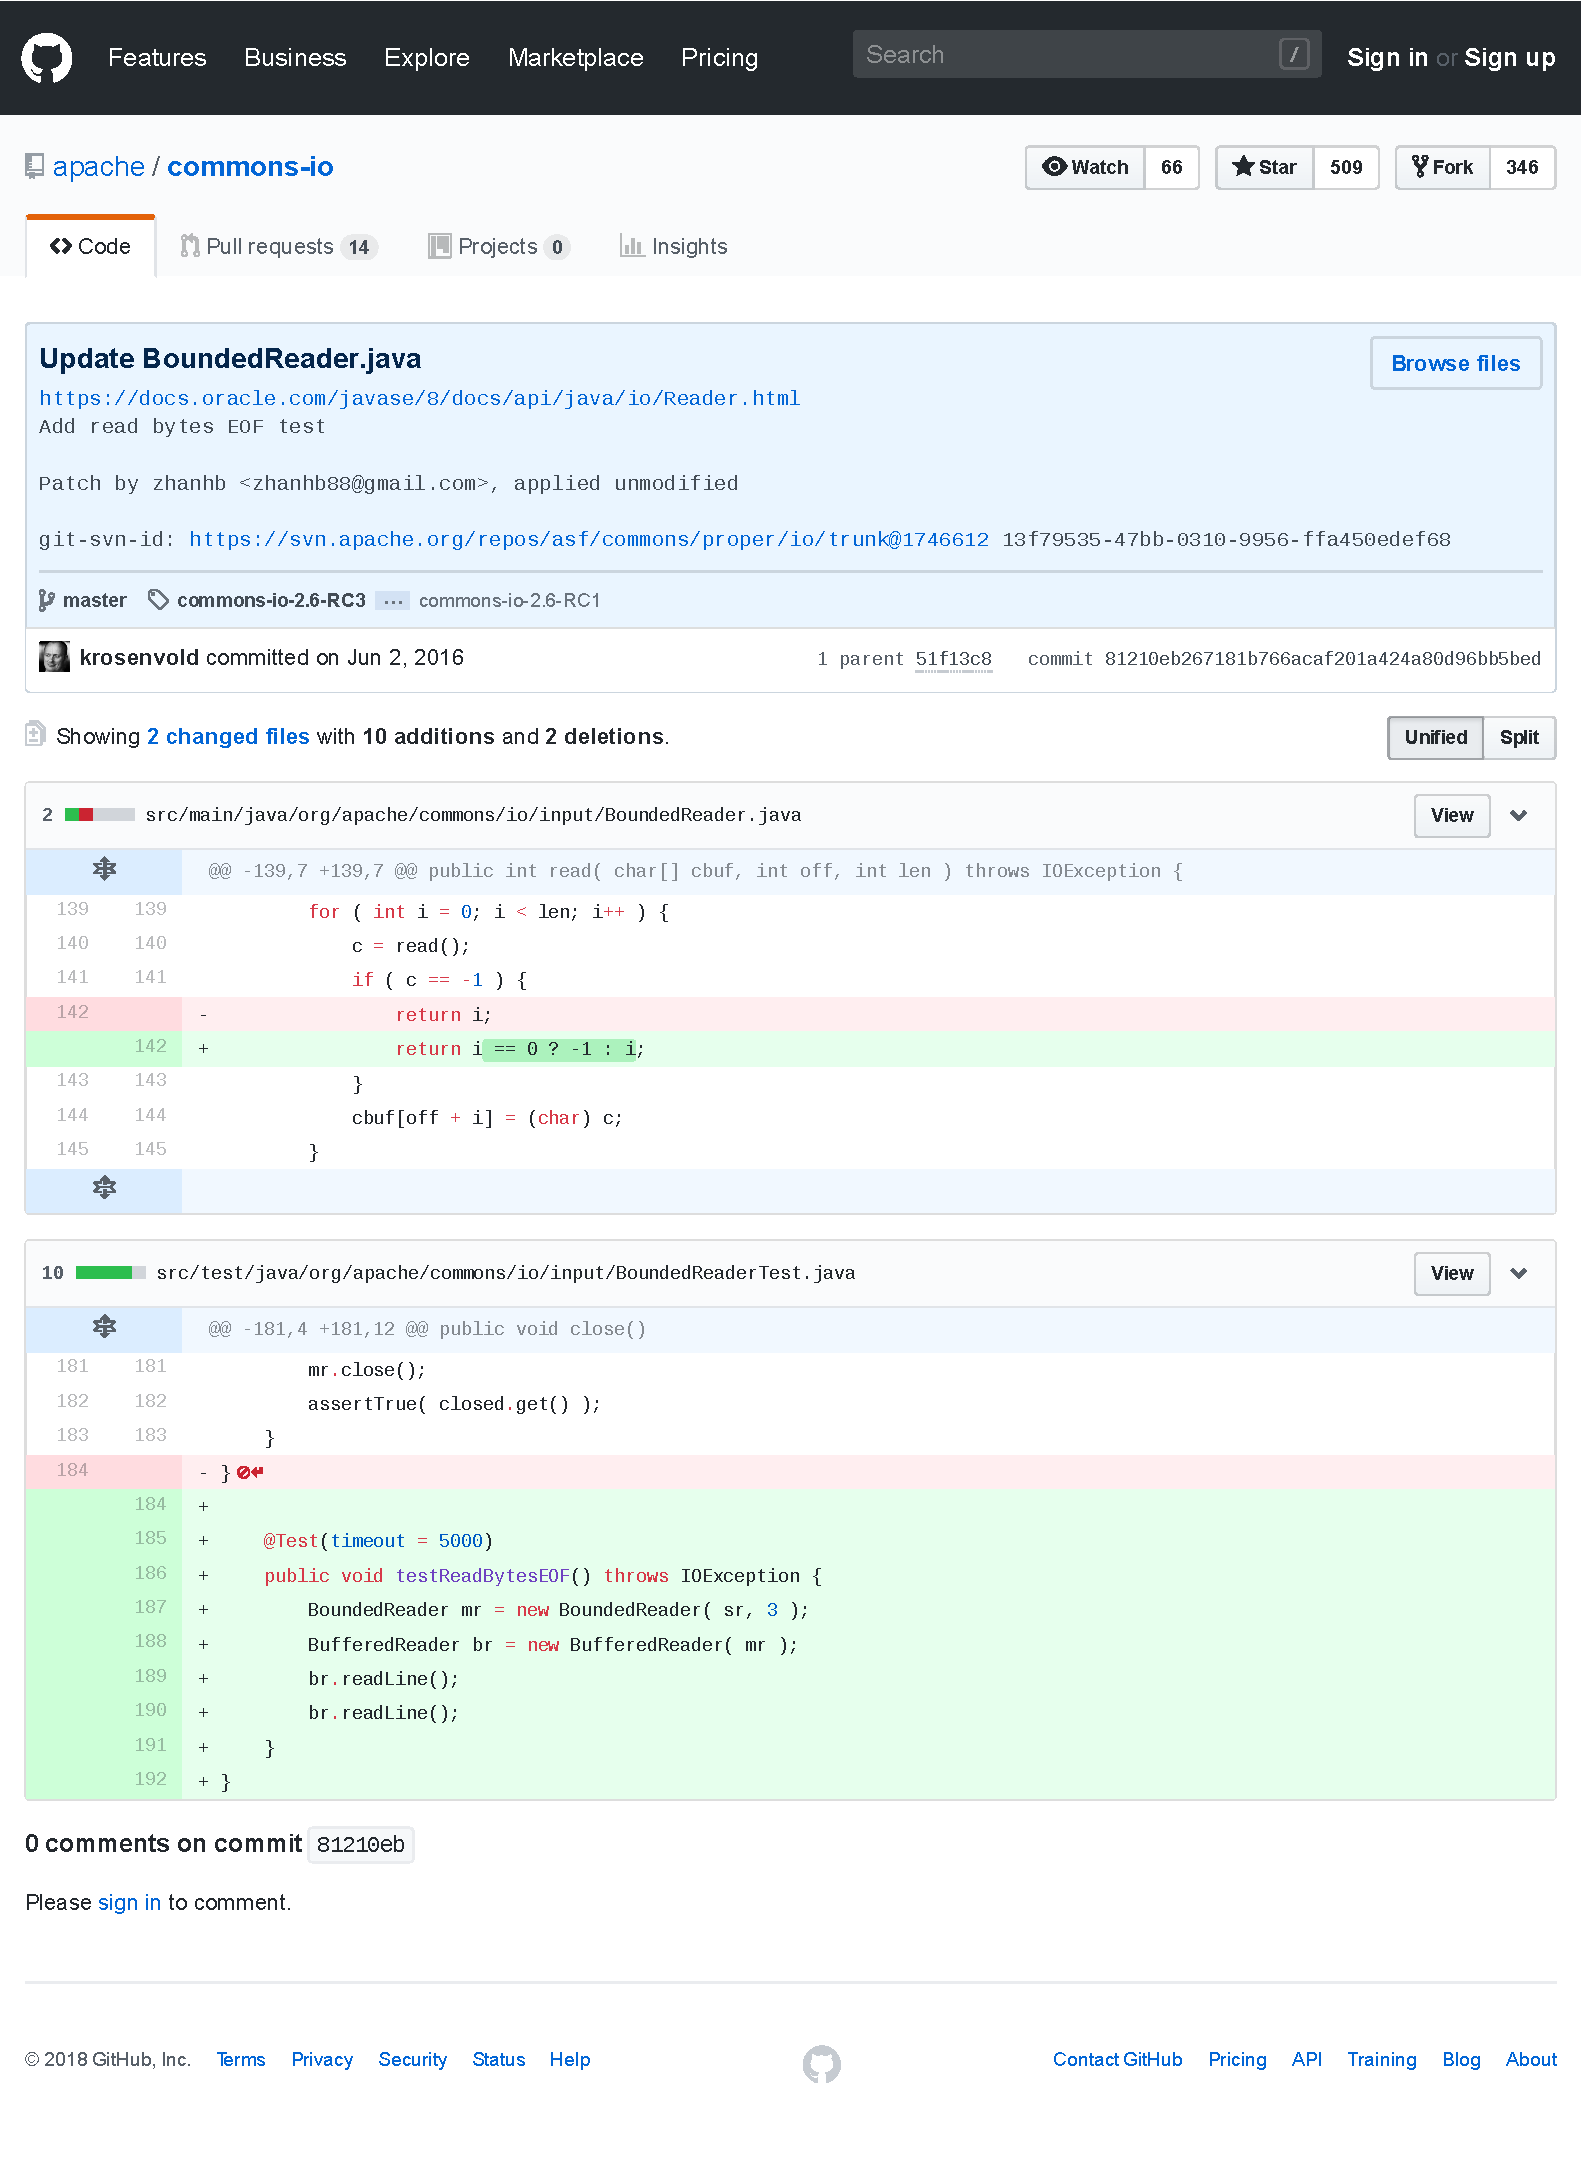
\includegraphics[width=.97\linewidth, trim=4cm 6.7cm 12.6cm 25.8cm, clip]{img/diff/diff-commons-io.pdf}}
\caption{Developer test for commit \textsc{81210eb} of commons-io.}
\label{fig:diff_commons-io}
\end{figure}


%%% COMMONS LANG
\textsc{commons-lang\#e7d16c2}\footnote{\url{https://github.com/apache/commons-lang/commit/e7d16c2}}: this commit escapes special characters before adding them to a \texttt{StringBuffer}.
\autoref{fig:ampl_commons-lang} shows the amplified test method obtained by \DCII.
The assertion at the bottom of the excerpt is the one that detects the behavioral change.
This assertion compares the content of the \texttt{StringBuilder} against an expected string.
In the pre-commit version, no special character is escaped, \eg '\textbackslash n'.
In the post-commit version, the DCI test fails since the code now escapes the special character \textbackslash.

\begin{figure}[h]
\centering
\fbox{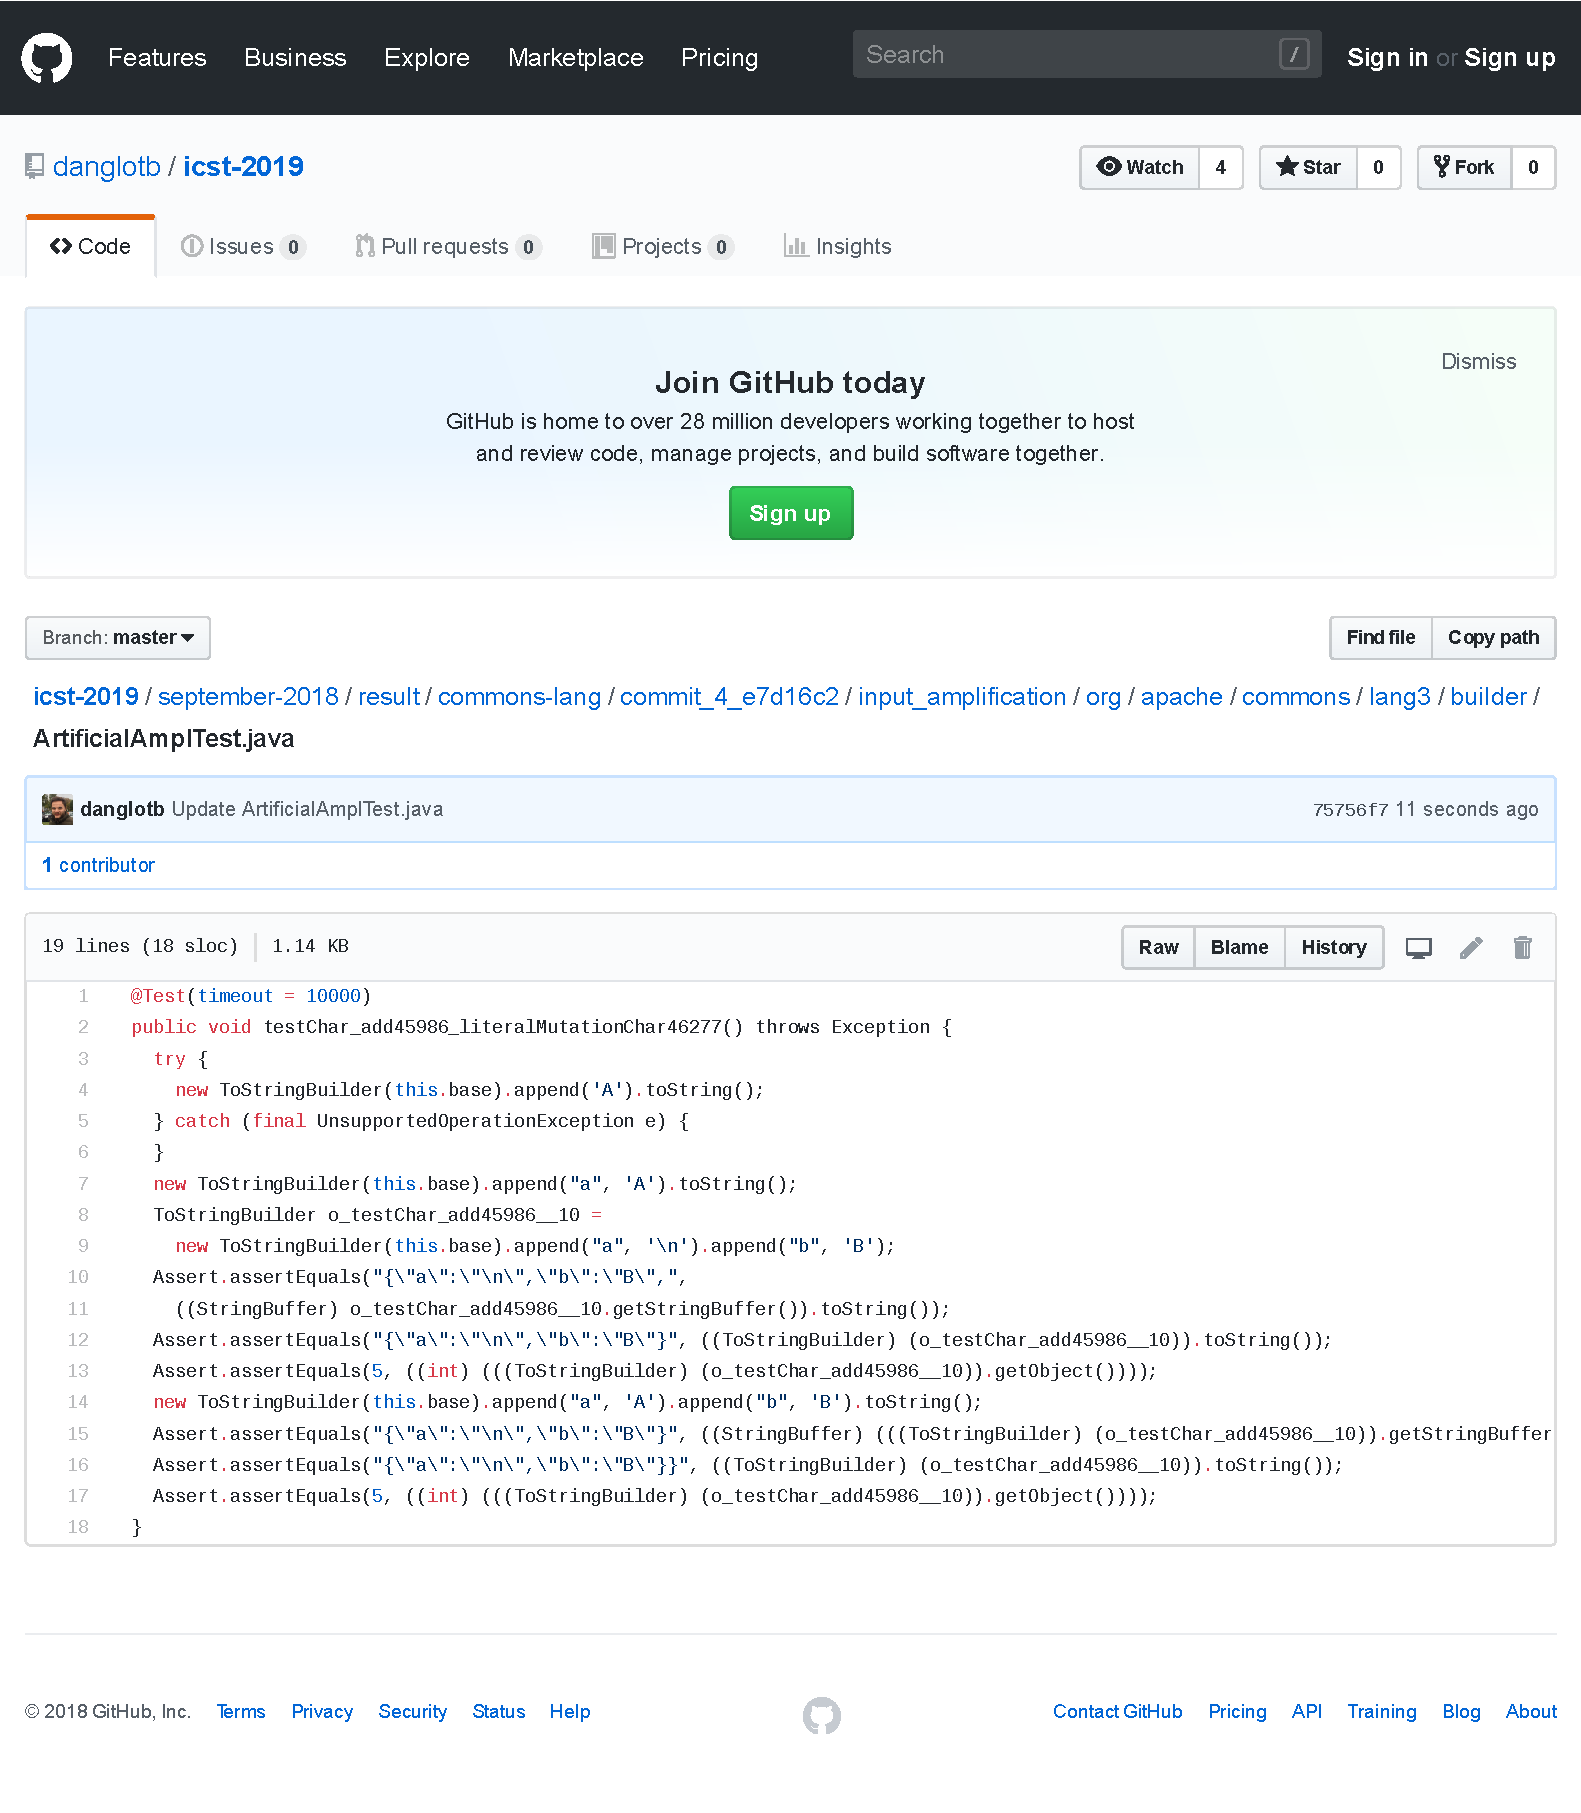
\includegraphics[width=.97\linewidth, trim=2.6cm 8.35cm 10.8cm 20.85cm, clip ]{img/amplified/ampl-commons-lang.pdf}}
\caption{Test generated by \DCII that detects the behavioral change of \textsc{e7d16c2} in commons-lang.}
\label{fig:ampl_commons-lang}
\end{figure}

Let's have a look to the human test method shown in \autoref{fig:diff_commons-lang}.
Here, the developer specified the new escaping mechanism with 5 different inputs.
%
The main difference between the human test and the amplified test is that the human test is more readable and uses 5 different inputs.
However, the amplified test generated by DCI is valid since it detects the behavioral change correctly.

\begin{figure}[h]
\centering
\fbox{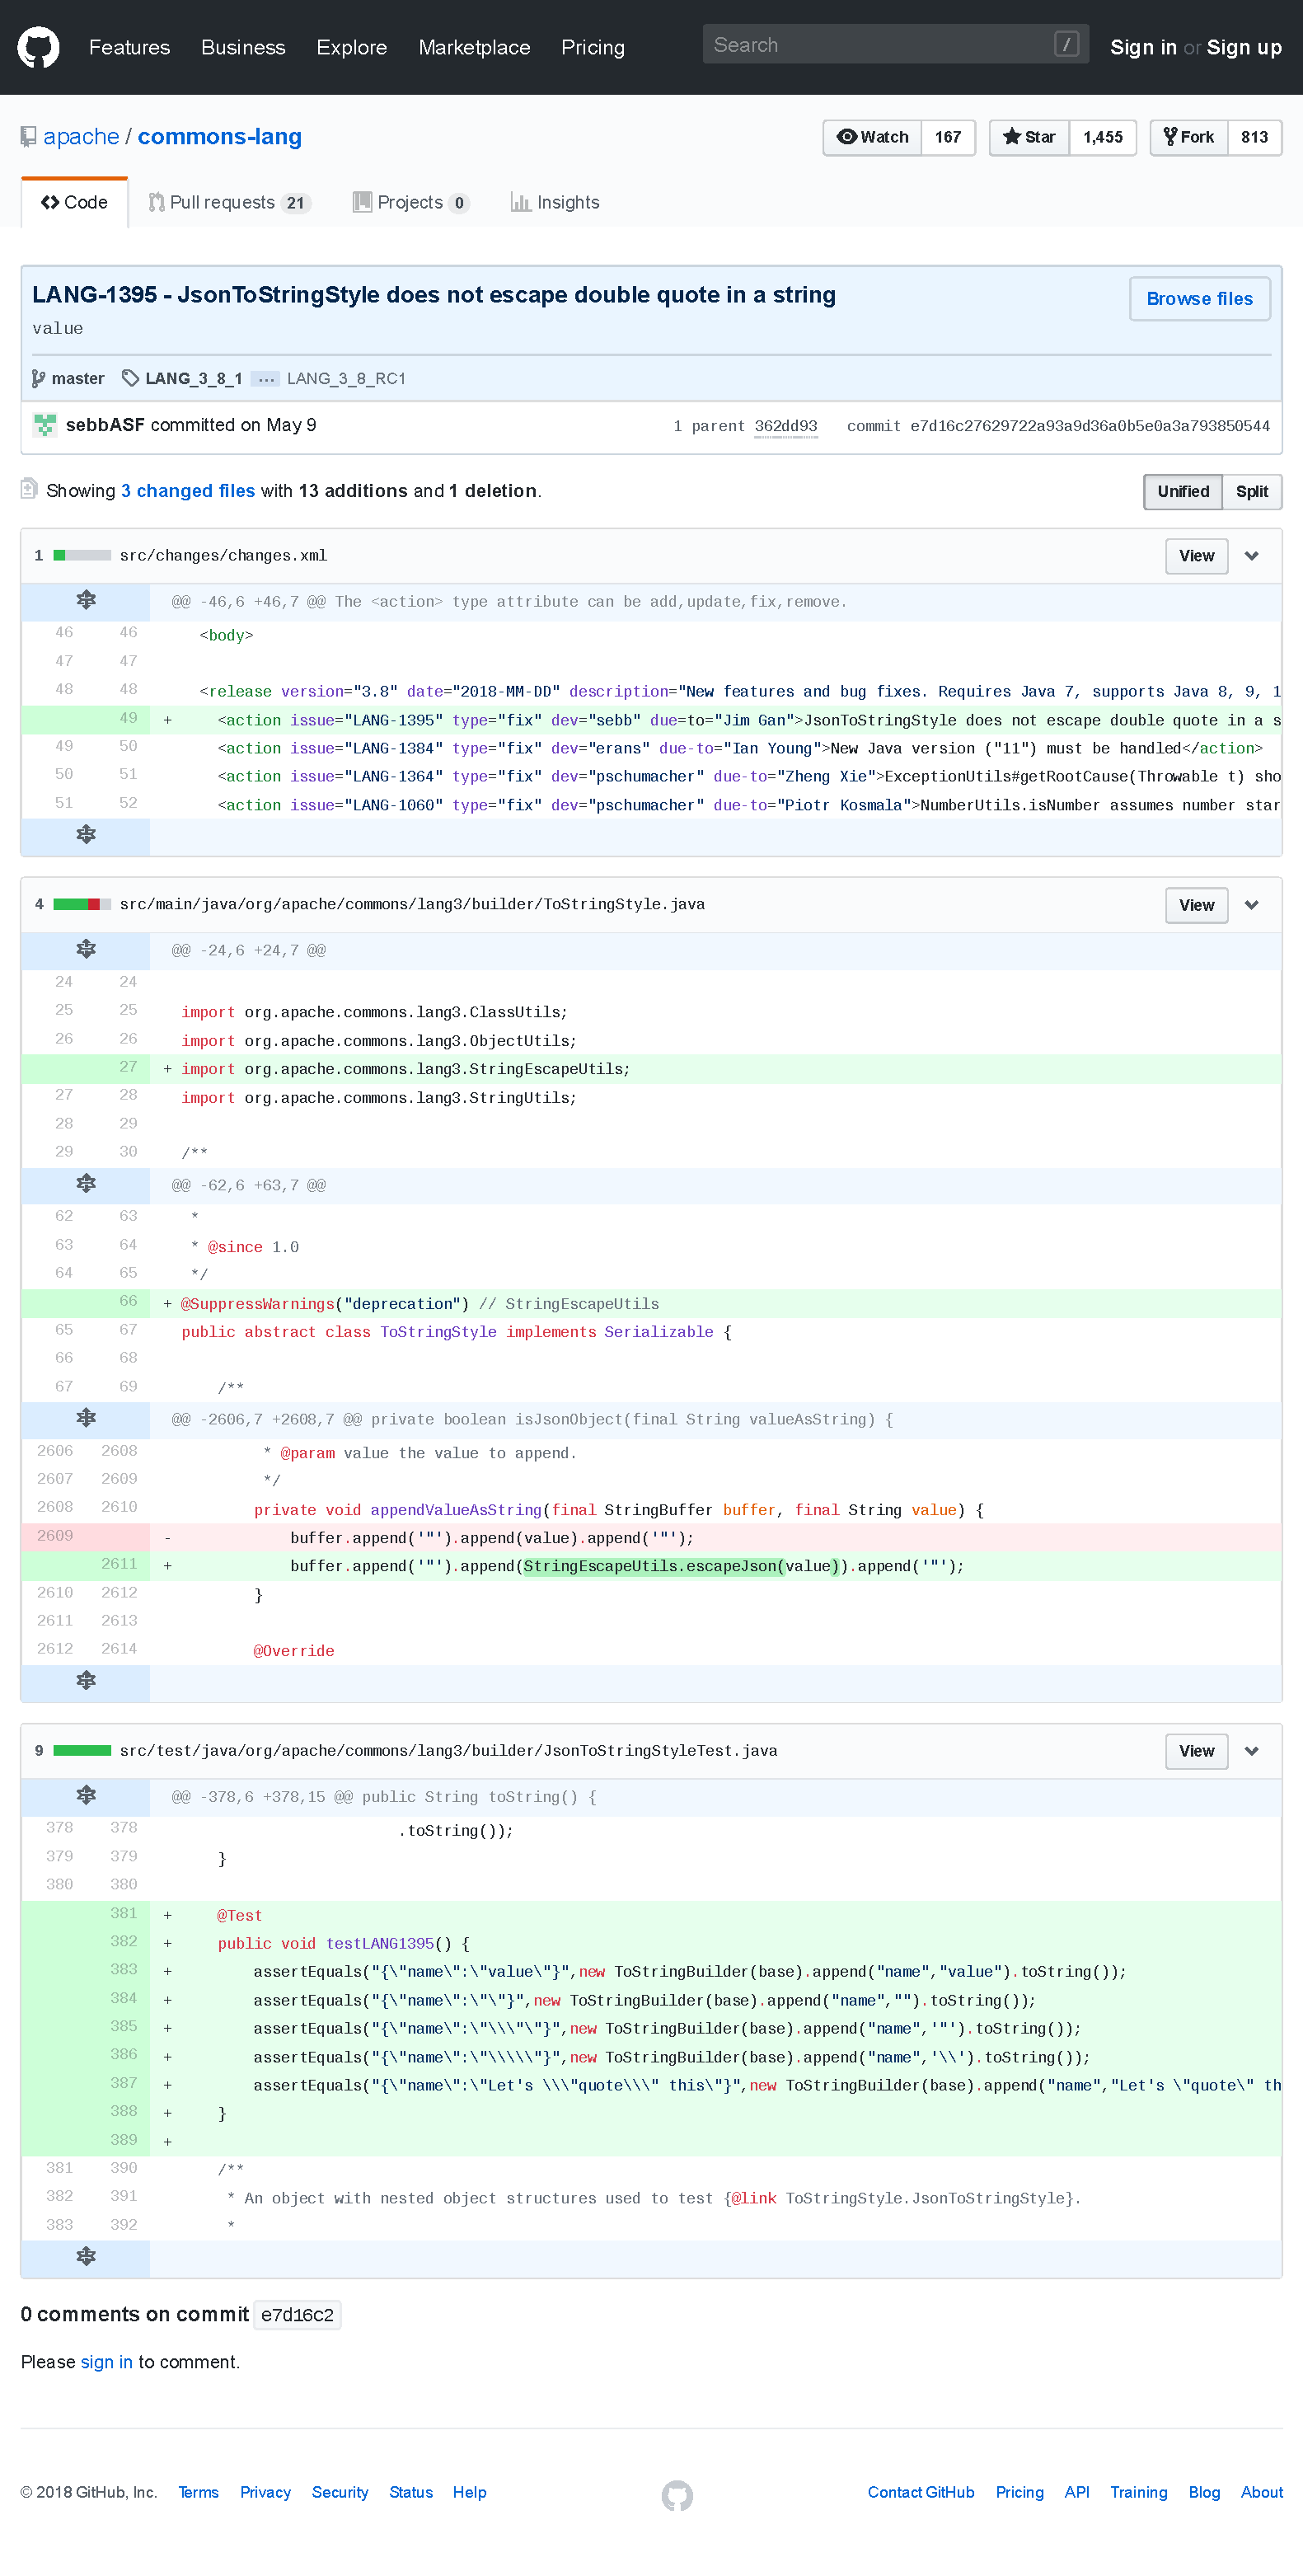
\includegraphics[width=.97\linewidth, trim=4.5cm 9.2cm 5.8cm 39.2cm, clip]{img/diff/diff-commons-lang.pdf}}
\caption{Developer test for \textsc{e7d16c2} of commons-lang.}
\label{fig:diff_commons-lang}
\end{figure}


%% GSON
\textsc{gson\#44cad04}\footnote{\url{https://github.com/google/gson/commit/44cad04}}: This commit allows Gson to deserialize a number represented as a string.
\autoref{fig:ampl_gson} shows the relevant part of the test generated by DCI$_{SBAMPL}$, based on \texttt{testNumberDeserialization} of \texttt{PrimitiveTest} as a seed.
First, we see that the test selected as a seed is indeed related to the change in the deserialization feature.
The DCI test detects the behavioral change at lines 3 and 4.
On the pre-commit version, line 3 throws a \texttt{JsonSyntaxException}.
On the post-commit version, line 4 throws a \texttt{NumberFormatException}.
In other words, the behavioral change is detected by a different exception (different type and not thrown at the same line).
\footnote{Interestingly, the number is parsed lazily, only when needed. Consequently, the exception is thrown when invoking the \texttt{longValue()} method and not when invoking \texttt{parse()}}.

\begin{figure}[h]
\centering
\fbox{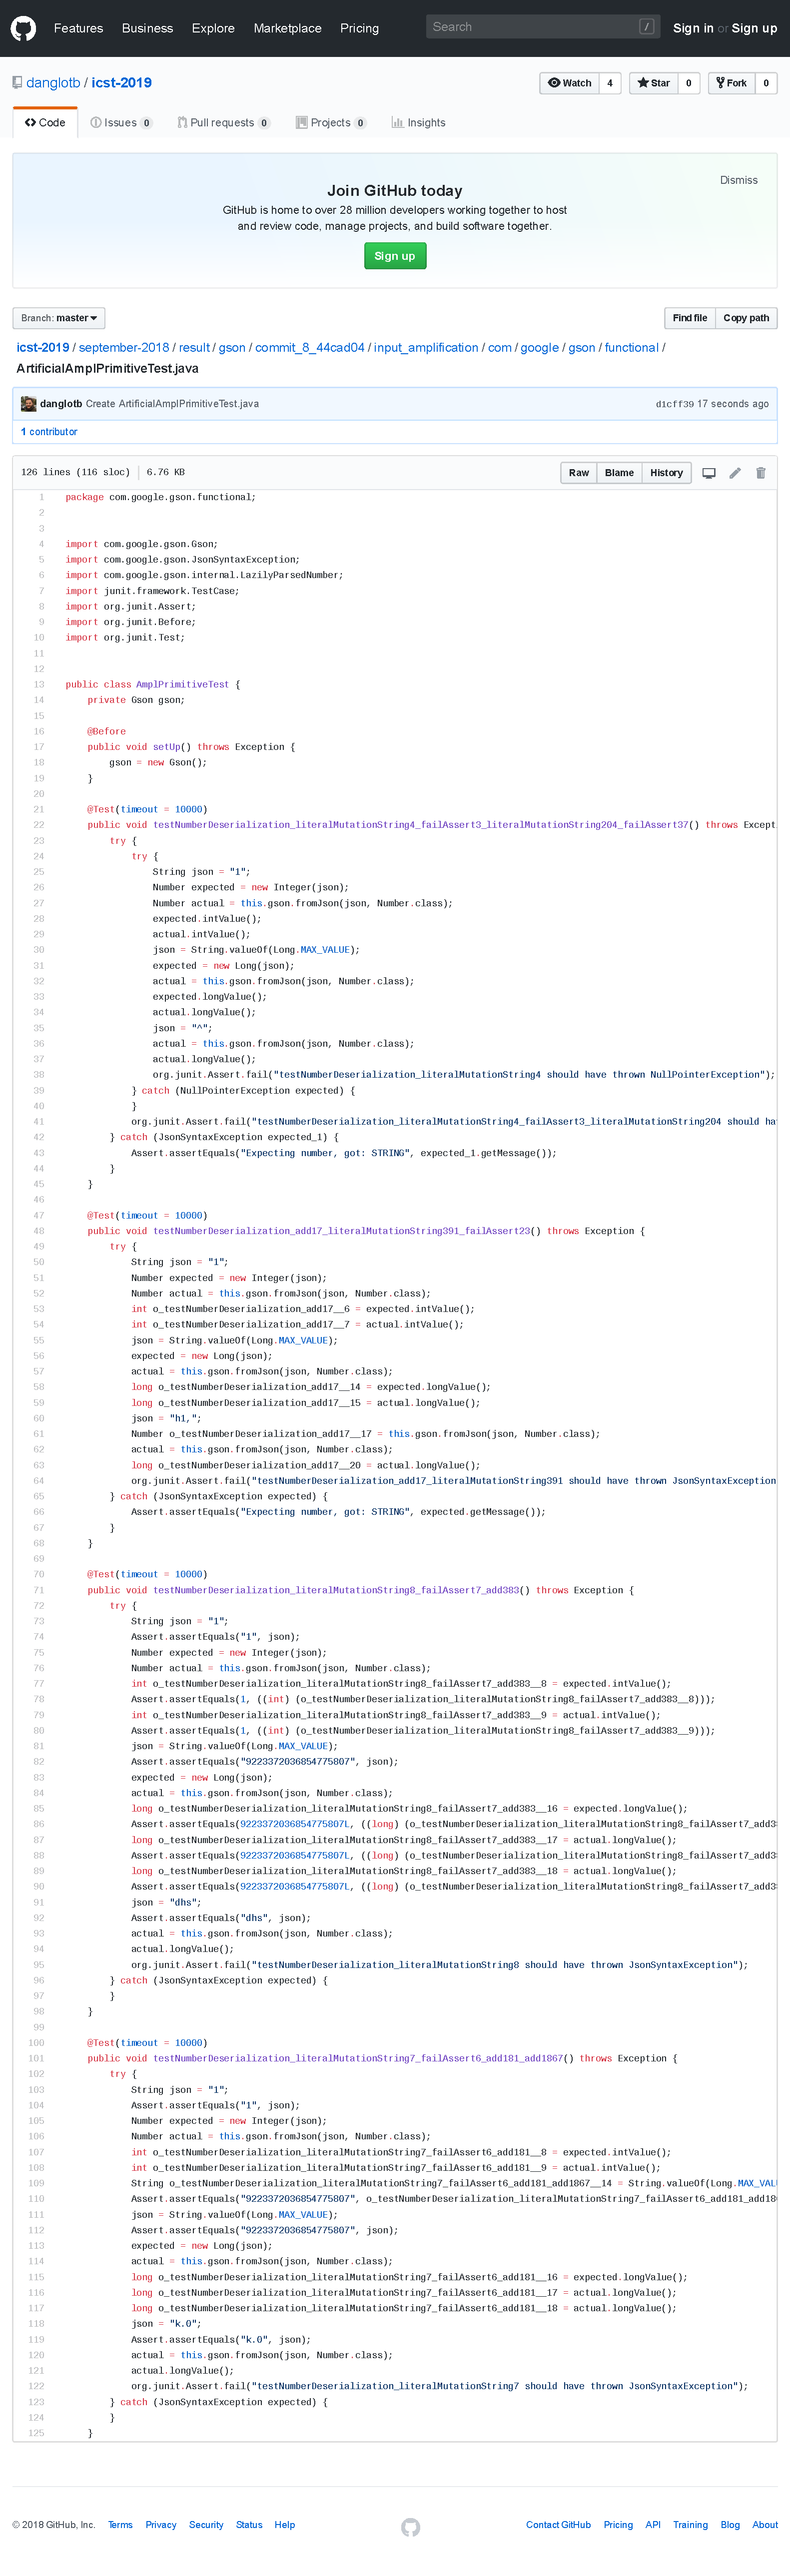
\includegraphics[width=.95\linewidth, trim=3.7cm 19.5cm 13.4cm 64.2cm, clip]{img/amplified/ampl-gson.pdf}}
\caption{Test generated by DCI that detects the behavioral change of commit \textsc{44cad04} in Gson.}
\label{fig:ampl_gson}
\end{figure}

We compare it against the developer-written ground-truth method, shown in \autoref{fig:diff_gson}. 
This short test verifies that the program handles a number-as-string correctly.
For this example, the DCI test does indeed detect the behavioral change, but in an indirect way.
On the contrary, the developer test is shorter and directly targets the changed behavior, which is better.

\begin{figure}[h]
\centering
\fbox{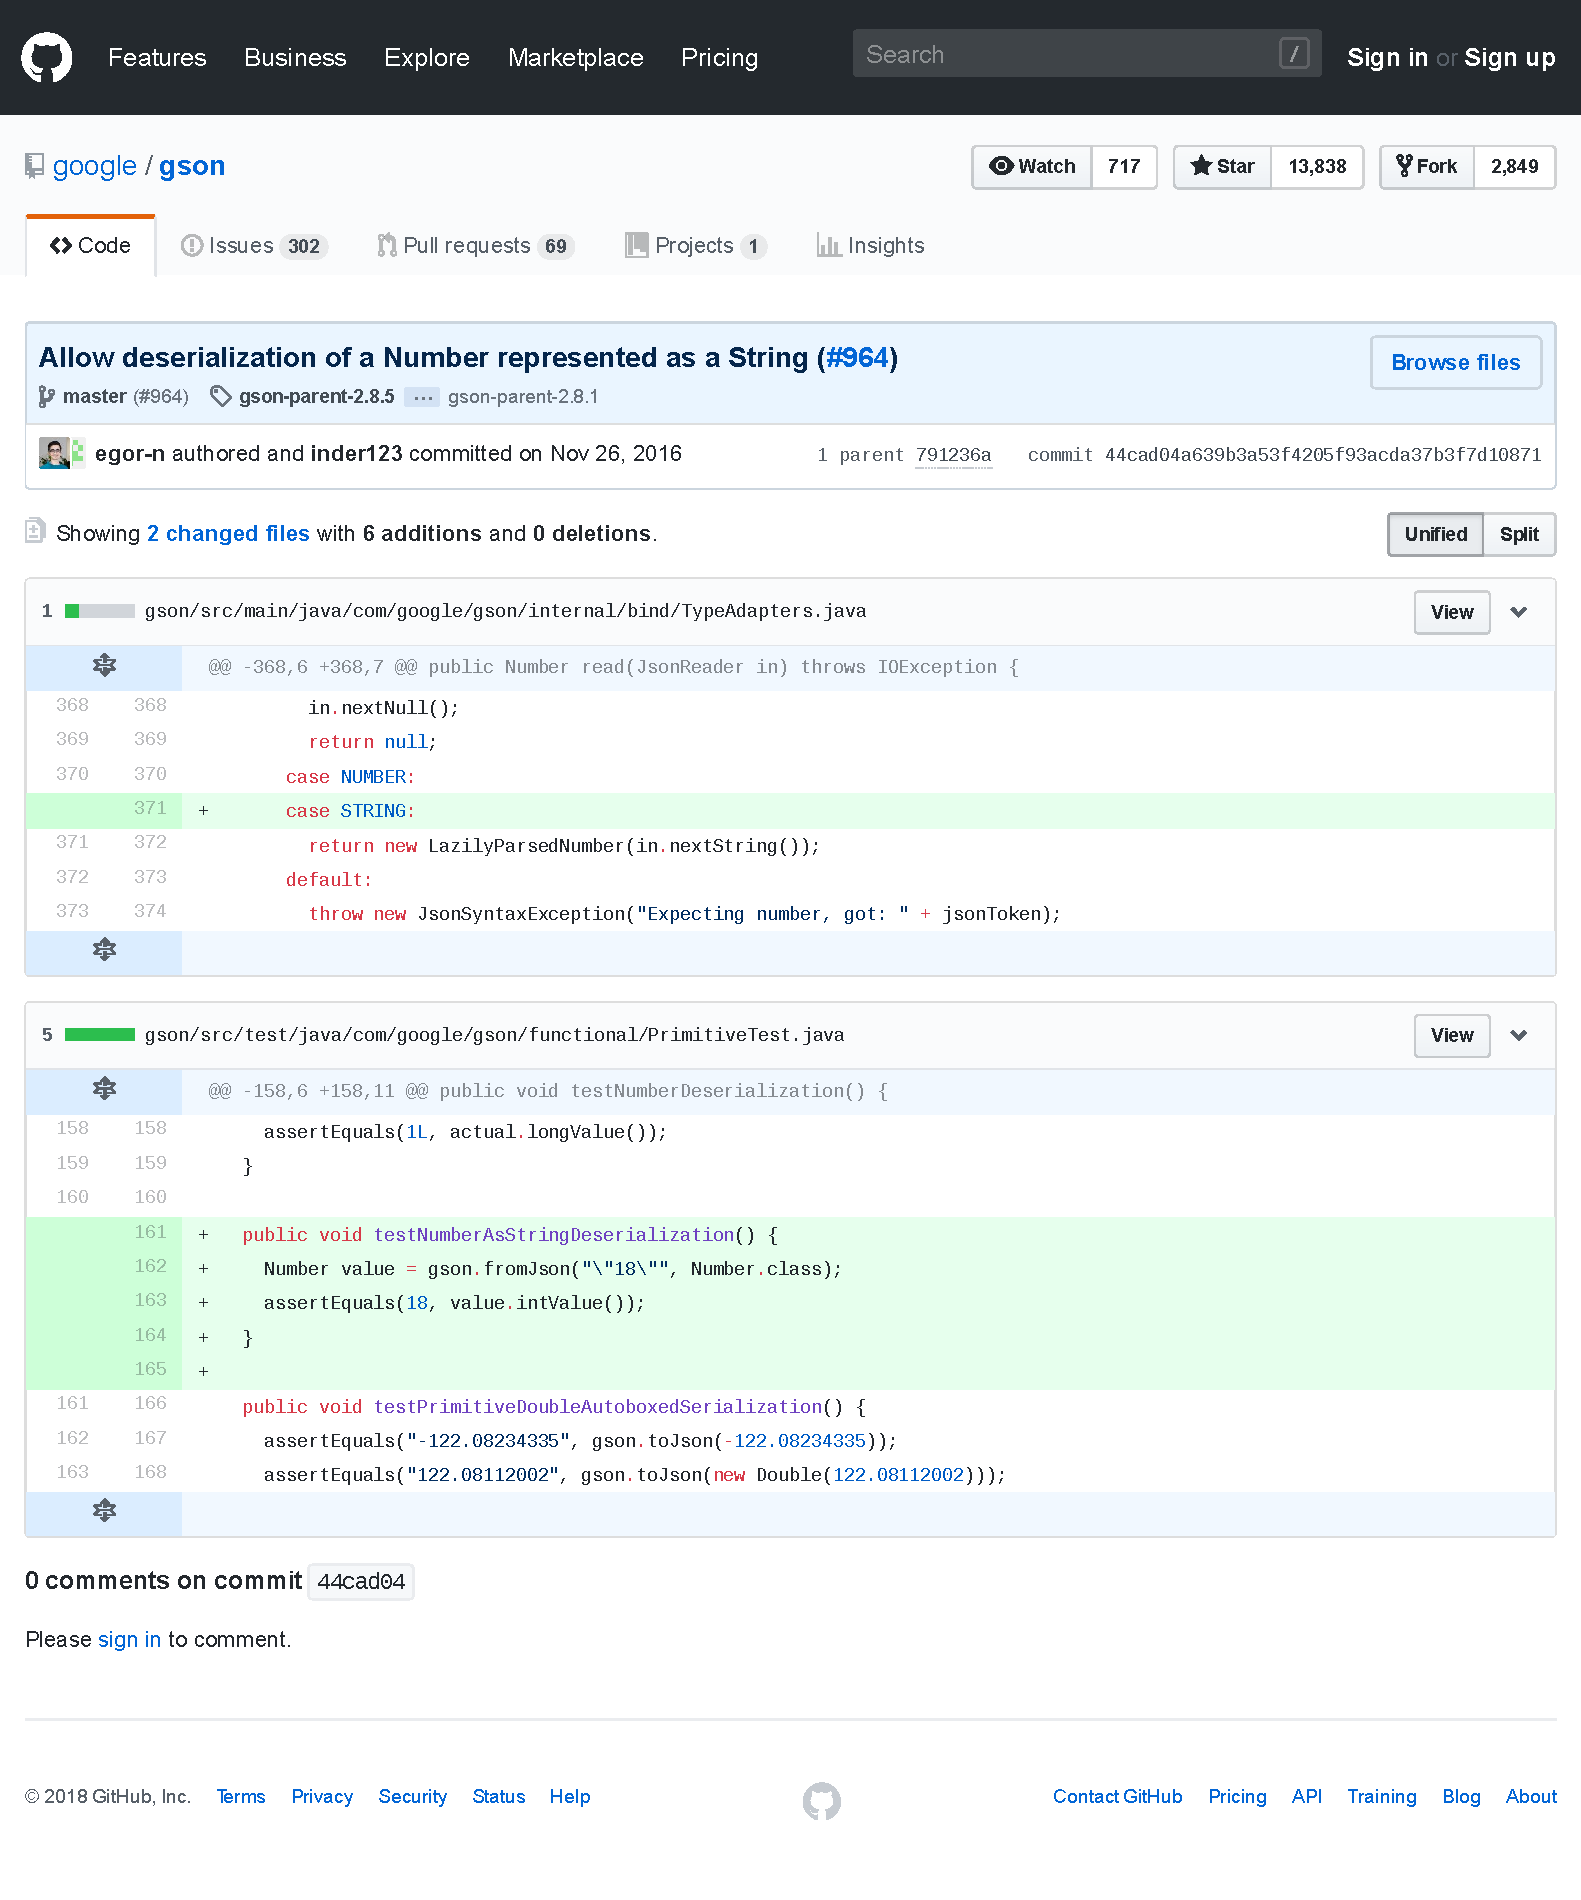
\includegraphics[width=.95\linewidth, trim=4cm 9.3cm 12.5cm 20.6cm ,clip]{img/diff/diff-gson.pdf}}
\caption{Provided test by the developer for \textsc{44cad04} of Gson.}
\label{fig:diff_gson}
\end{figure}



%% JSOUP
\textsc{jsoup\#3676b13}\footnote{\url{https://github.com/jhy/jsoup/commit/3676b13}}: This change is a pull request (\ie a set of commits) and introduces 5 new behavioral changes. There are two improvements: skip the first new lines in pre tags and support deflate encoding, and three bug fixes: throw exception when parsing some urls, add spacing when output text, and no collapsing of attribute with empty values.
\autoref{fig:ampl_jsoup} shows an amplified test obtained using \DCII.
This amplified test has 15 assertions and a duplication of method call.
Thanks to this duplication and assertion generated on the \texttt{toString()} method, this test is able to capture the behavioral change introduced by the commit.

\begin{figure}[h]
\centering
\fbox{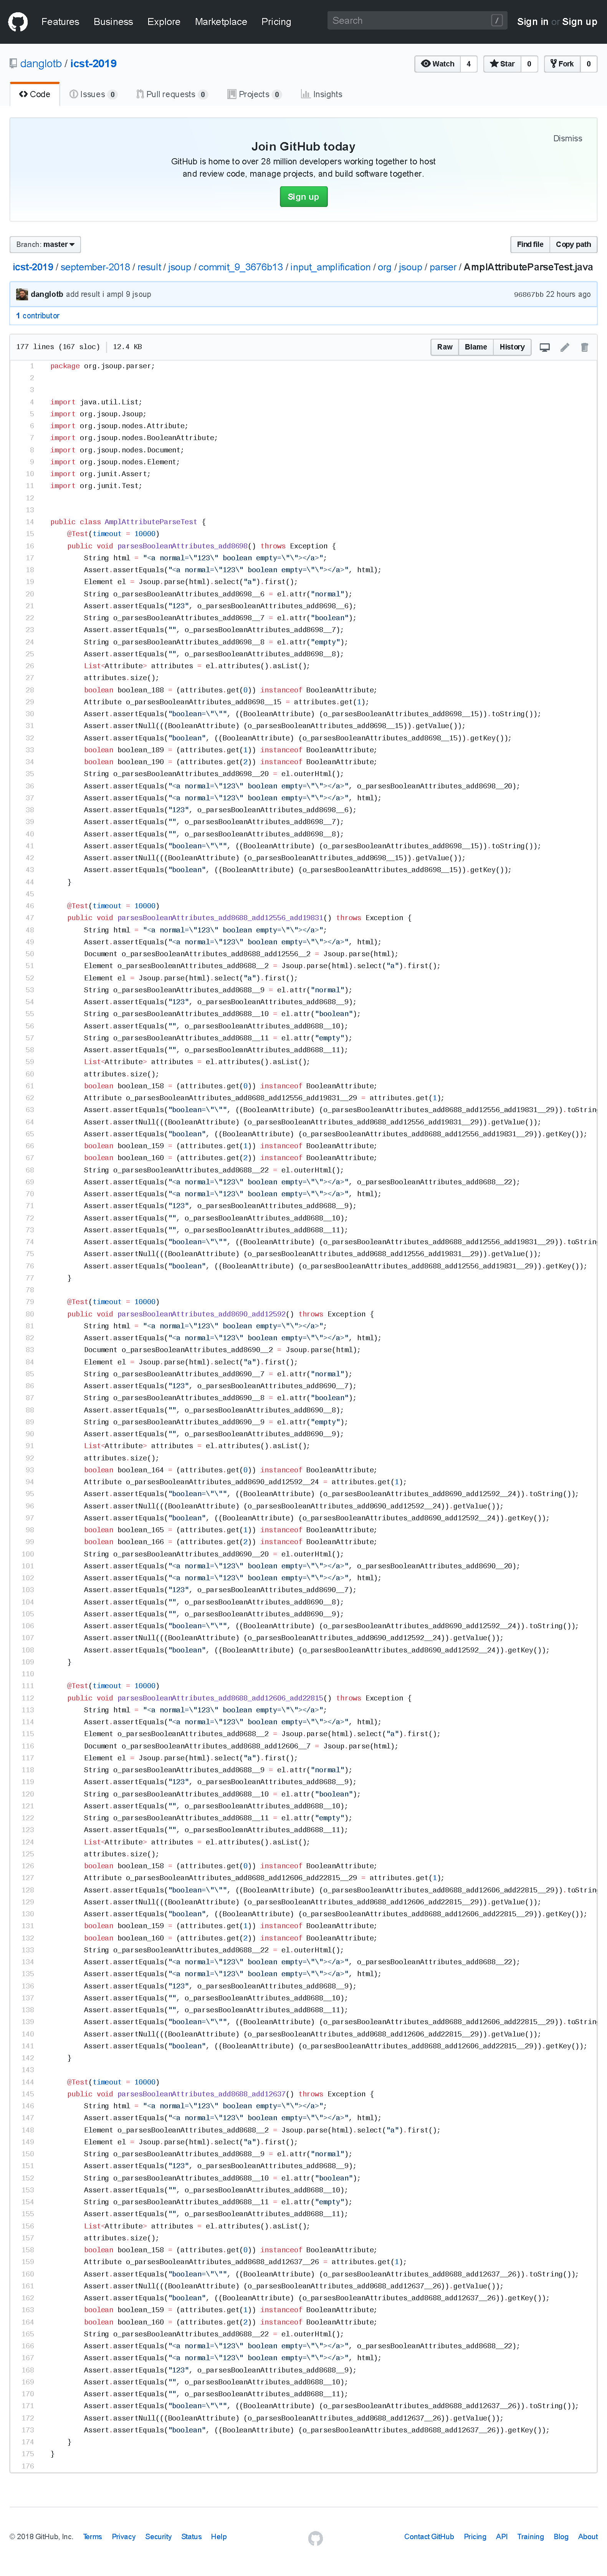
\includegraphics[width=.95\linewidth, trim=3.7cm 82cm 7cm 30.8cm ,clip]{img/amplified/ampl-jsoup.pdf}}
\caption{Test generated by \DCII that detects the behavioral change of \textsc{3676b13} of Jsoup.}
\label{fig:ampl_jsoup}
\end{figure}

As before, we compare it to the developer's test. 
The developer uses the \texttt{Element} and \texttt{outerHtml()} methods rather than \texttt{Attribute} and \texttt{toString()}.
However, the method \texttt{outerHtml()} in \texttt{Element} will call the \texttt{toString()} method of \texttt{Attribute}.
For this behavioral change, it concerns the \texttt{Attribute} and not the \texttt{Element}.
So, the amplified test is arguably better, since it is closer to the change than the developer's test.
But, \DCII generates amplified tests that detect 2 of 5 behavioral changes: adding spacing when output text and no collapsing of attribute with empty values only, so regarding the quantity of changes, the human tests are more complete.

\begin{figure}[h]
\centering
\fbox{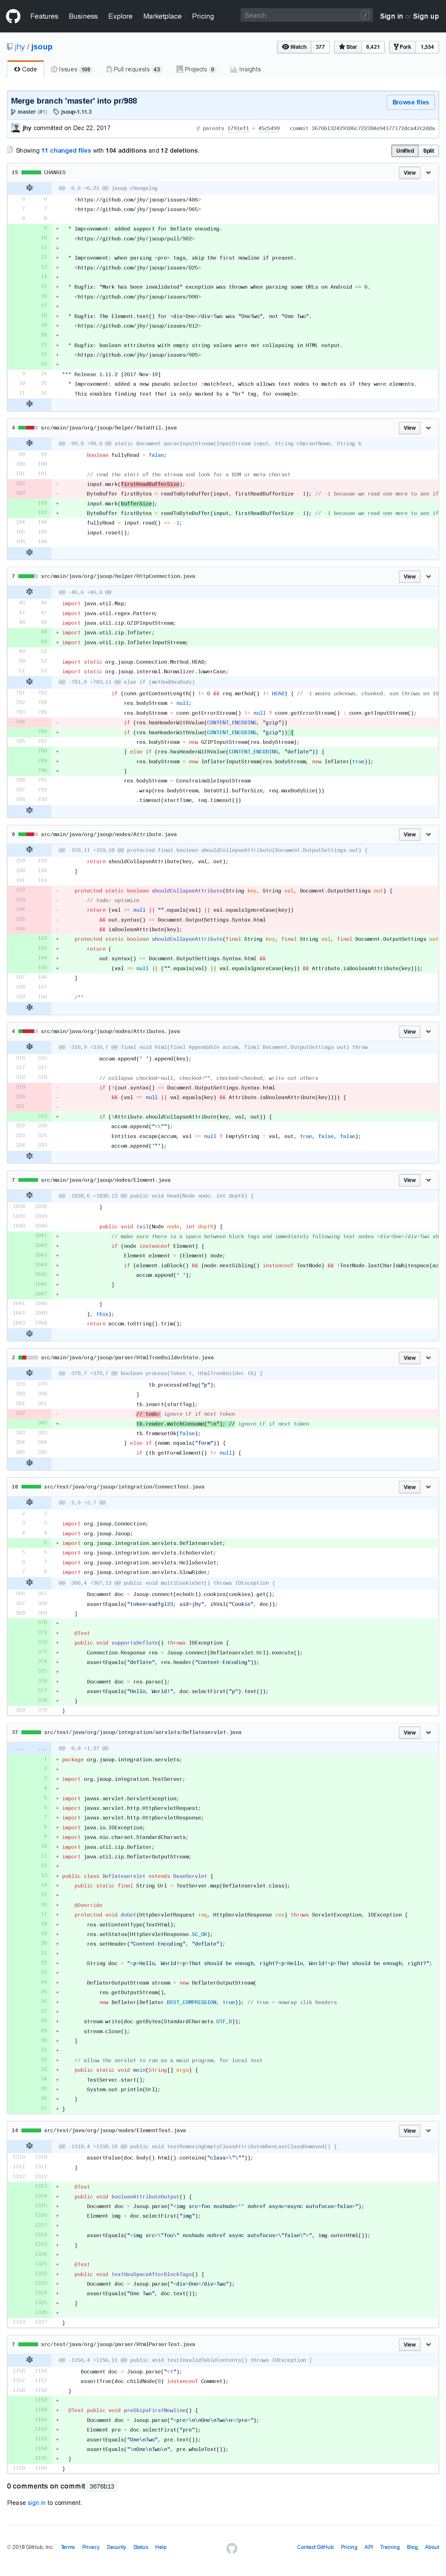
\includegraphics[width=.95\linewidth, trim=4.3cm 19.6cm 4.8cm 131.5cm , clip]{img/diff/diff-jsoup.pdf}}
\caption{Provided test by the developer for \textsc{3676b13} of Jsoup.}
\label{fig:diff_jsoup}
\end{figure}

%%%%%%%%%%%%%%%%%%%%%%%%%%%%%%%%%%%%%%%
%% MUSTACHE JAVA
\textsc{Mustache.java\#774ae7a}\footnote{\url{https://github.com/spullara/mustache.java/commit/774ae7a}}: This commit fixes an issue with the usage of a dot in a  relative path on Window in the method \texttt{getReader} of class \texttt{ClasspathResolver}.
The test method \texttt{getReaderNullRootDoesNotFindFileWithAbsolutePath} has been used as seed by DCI. It modifies the existing string literal with another string used somewhere else in the test class and generates 3 new assertions.
The behavioral change is detected thanks to the modified strings: it produces the right test case containing a space.

\begin{figure}[h]
\centering
\fbox{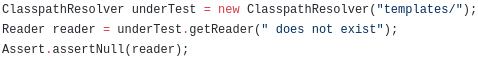
\includegraphics[width=.95\linewidth]{img/amplified/ampl-mustache.png}}
\caption{Test generated by \DCII that detects the behavioral change of \textsc{774ae7a} of Mustache.java.}
\label{fig:ampl_mustache}
\end{figure}

The developer proposed two tests that verify that the object reader is not null when getting it with dots in the path.
There are shown in \autoref{fig:diff_mustache}.
These tests invoke the method \texttt{getReader} which is the modified method in the commit.
%
The difference is that the \DCII's amplified test method provides a non longer valid input for the method \texttt{getReader}.
However, providing such inputs produce errors afterward which signal the behavioral change.
In this case, the amplified test is complementary to the human test since it verifies that the wrong inputs are no longer supported and that the system immediately throws an error.

\begin{figure}[h]
\centering
\fbox{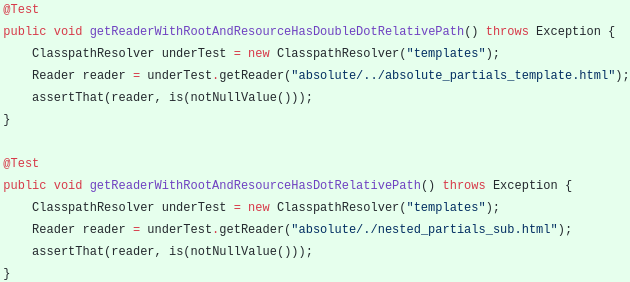
\includegraphics[width=.95\linewidth]{img/diff/diff-mustache.png}}
\caption{Developer test for \textsc{774ae7a} of Mustache.java.}
\label{fig:diff_mustache}
\end{figure}

%%%%%%%%%%%%%%%%%%%%%%%%%%%%%%%%%%%%%%%
%% XWIKI COMMONS
\textsc{xwiki-commons\#d3101ae}\footnote{\url{https://github.com/xwiki/xwiki-commons/commit/d3101ae}}: This commit fixes a bug in the \texttt{merge} method of class \texttt{DefaultDiffManager}.
\autoref{fig:ampl_xwiki} shows the amplified test method obtained by \DCIA.
DCI used \texttt{testMergeCharList} as a seed for the amplification process, and generates 549 new assertions.
Among them, 1 assertion captures the behavioral change between the two versions of the program: 
``assertEquals(0, result.getLog().getLogs(LogLevel.ERROR).size());''.
The behavioral change that is detected is the presence of a new logging statement in the diff. After verification, there is indeed such a behavioral change in the diff, with the addition of a call to ``logConflict'' in the newly handled case.

\begin{figure}[h]
\centering
\fbox{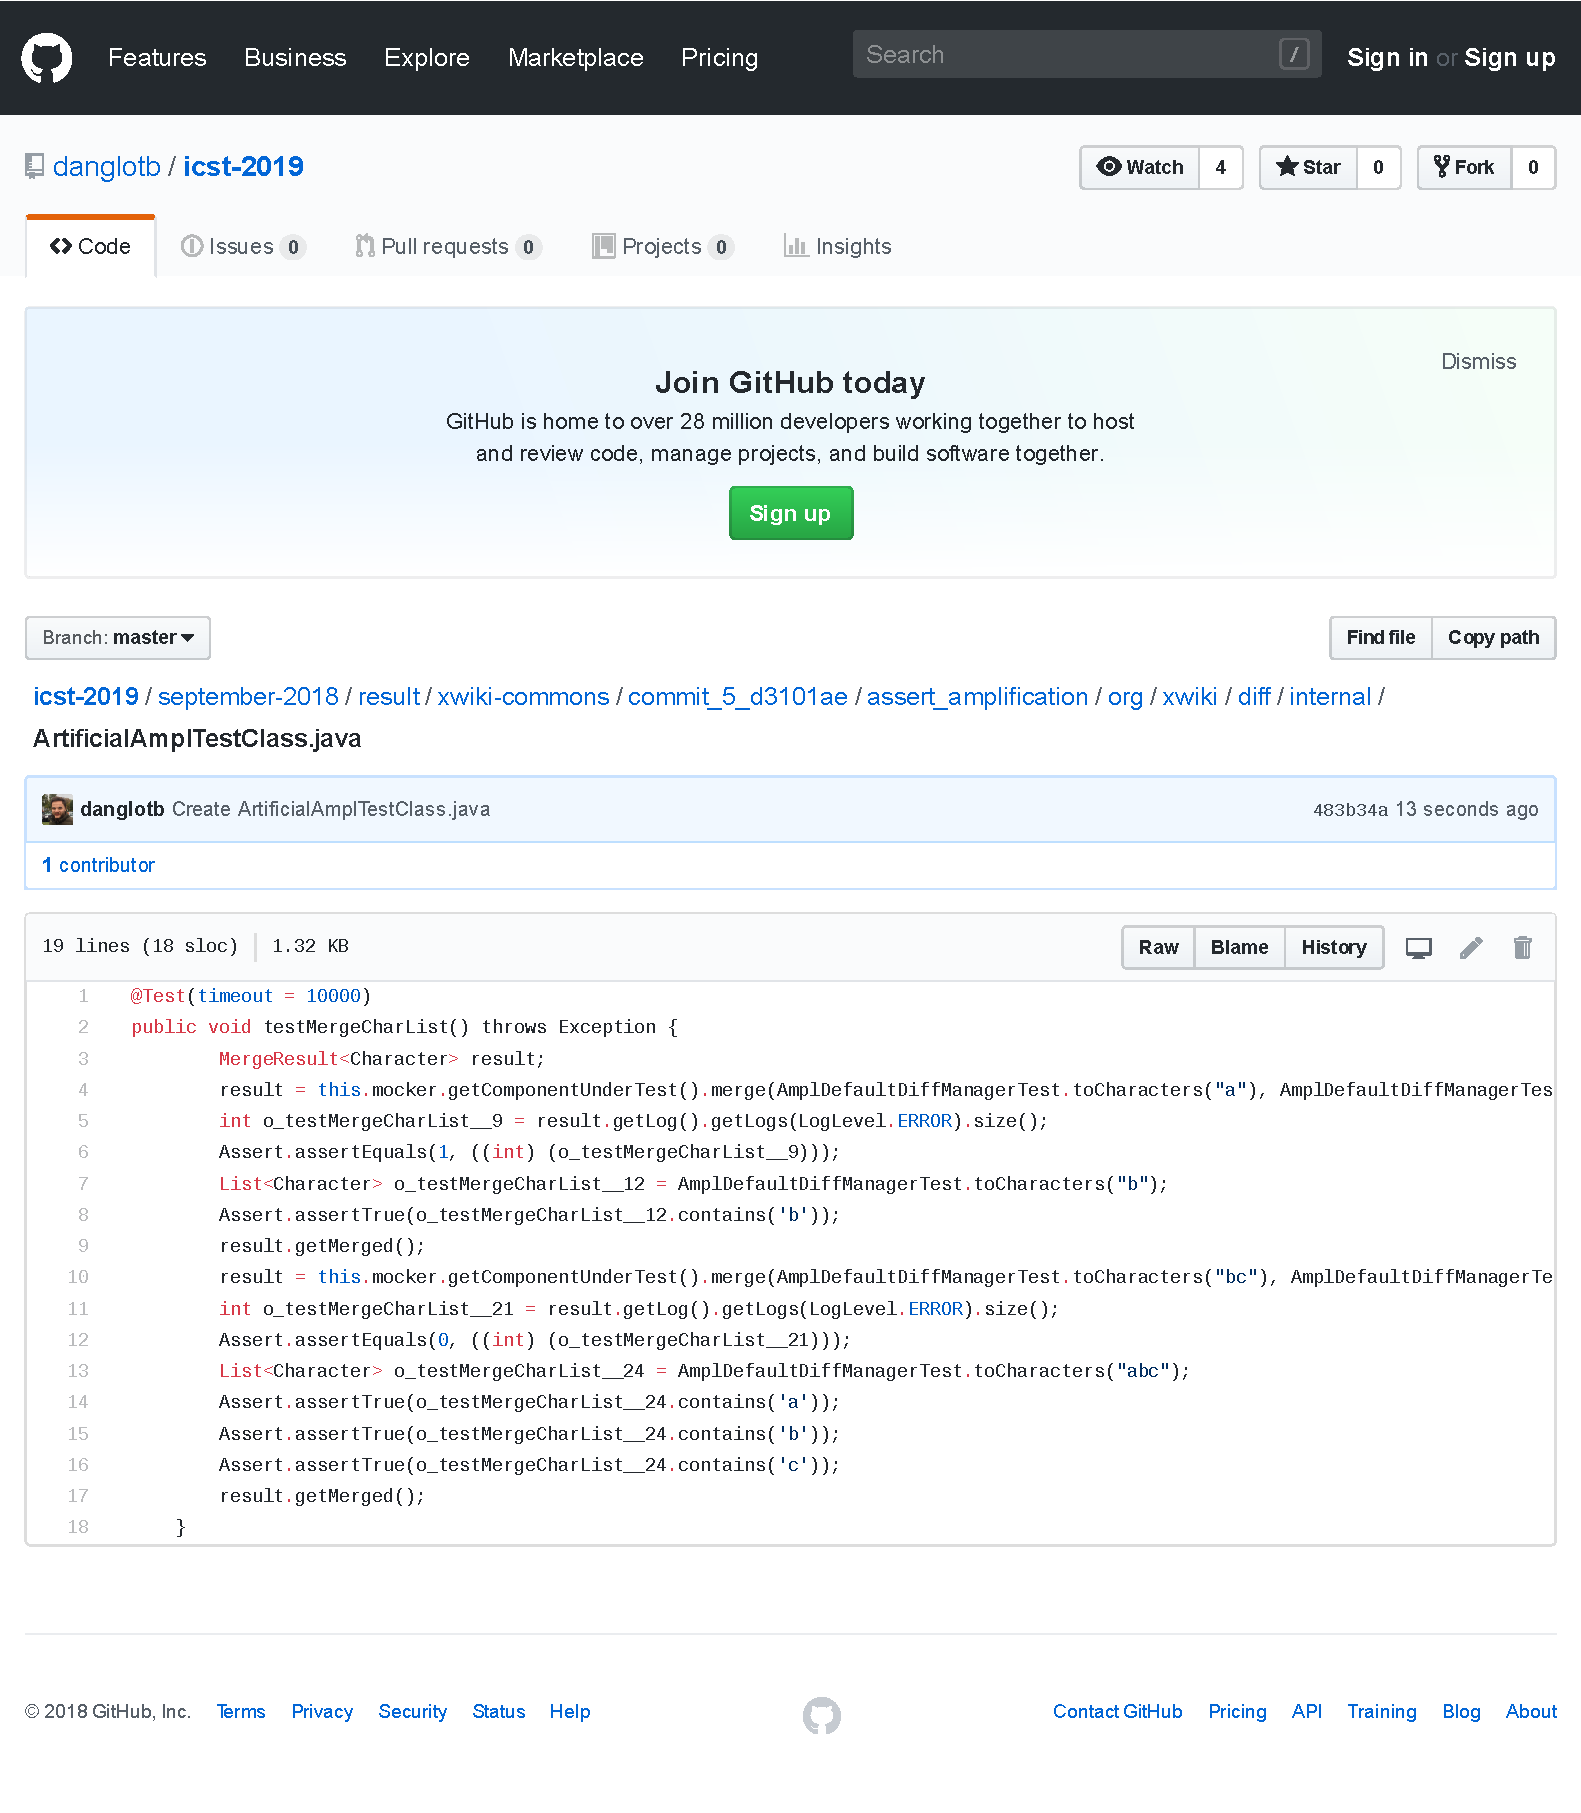
\includegraphics[width=.95\linewidth, trim=3.5cm 11.5cm 9.2cm 18.2cm, clip ]{img/amplified/ampl-xwiki.pdf}}
\caption{Test generated by \DCIA that detects the behavioral change of \textsc{d3101ae} of XWiki.}
\label{fig:ampl_xwiki}
\end{figure}

The developer's test is shown in \autoref{fig:diff_xwiki}.
This test method directly calls method \texttt{merge}, which is the method that has been changed. 
What is striking in this test is the level of clarity: the variable names, the explanatory comments and even the vertical space formatting are impossible to achieve with \DCIA and makes the human test clearly of better quality but also longer to write. % above when she has the time to write a good test. 
%
Yet, \DCIA's amplified tests capture a behavioral change that was not specified in the human test.
In this case, amplified tests can be complementary.

\begin{figure}[h]
\centering
\fbox{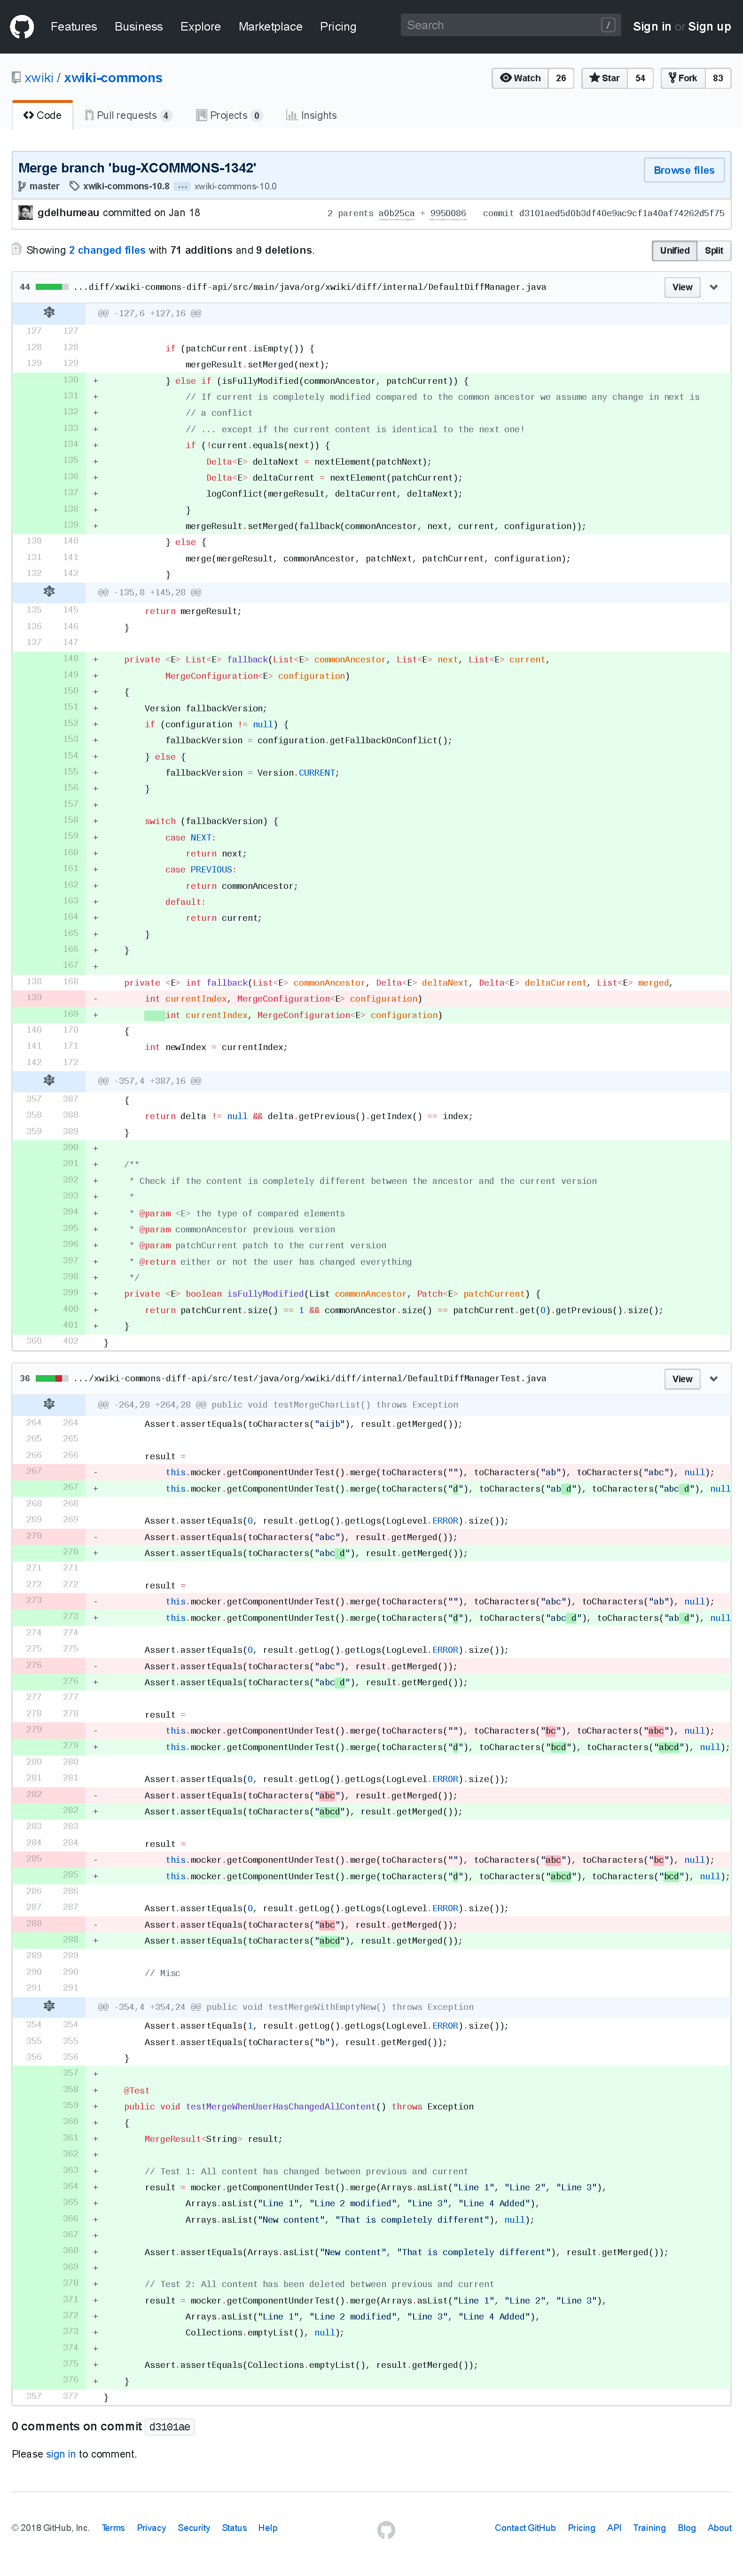
\includegraphics[width=.95\linewidth, trim=4.2cm 6.7cm 5cm 75cm, clip]{img/diff/diff-xwiki.pdf}}
\caption{Developer test for \textsc{d3101ae} of XWiki.}
\label{fig:diff_xwiki}
\end{figure}


\begin{mdframed}
Answer to \textbf{RQ4}: 
In 2 of 5 cases, the DCI test is complementary to the human test.
In 1 case, the DCI test can be considered better than the human test.
In 2 cases, the human test is better than the DCI test.
Even though human tests can be better, DCI can be complementary and catch missed cases, or can provide added-value when developers do not have the time to add a test.
\end{mdframed}

%\pagebreak


% -----------------------
%  Main Observed Limitation
% -----------------------
\section{Discussion about the scope of DCI}
\label{sec:limitation}

In this section, we overview the current limitations of DCI and the key factors that prevent DCI from amplifying test methods that detect behavioral changes.

\textbf{Time consumption}
From our experiments, we see that the time consumption to complete the amplification is the main limitation of DCI.
\textsc{jsoup\#2c4e79b}, almost 5 hours have been spent with no result.
For the sake of our experimentation, we choose to use a pre-defined number of iteration to bound the exploration.
In practice, we recommend to set a time budget (\eg at most one hour per pull-request).

\textbf{Importance of test seeds}
By construction, DCI's effectiveness is correlated to the test methods used as seed.
For example, see the row of \texttt{commons-lang\#c8e61af} in \autoref{tab:overall_result_iteration}
where one can observe that whatever the number of iteration, DCI takes the same time to complete the amplification.
The reason is that the seed tests are only composed of assertions statements.
Such tests are bad seeds for DCI and they prevent any good input amplification.

\textbf{False positive}
The risk of false positives is a potential  limitation of your approach.
A false positive would be an amplified test method that passes or fails on both versions, which means that the amplified test method does not detect the behavioral difference between both versions.
We manually  analyzed 6 commits and none of them are false positives.
While this is not a proof that DCI would never produce such confusing test methods, we are confident in the soundness of our implementation.

% -----------------------
%  THREATS
% -----------------------
\section{Threats to validity}
\label{sec:threats}

% bug in the implementation
An internal threat is the potential bugs in the implementation of DCI. However, we heavily tested our prototype with JUnit test cases to mitigate this threat.

% benchmark
In our benchmark, there are 60 commits. Our result may be not be generalizable to all programs. But we carefully selected real and diverse applications from GitHub, all having a strong test suite. We believe that the benchmark reflects real programs, and we have good confidence in the results.

% flaky amplified test
Last but not least threat is the potential flakiness of generated test methods.
However we take care that our approach does not produce flaky test methods, and we make sure to observe a stable and different state of the program between different executions. 
To do this, we execute 3 times each amplified test in order to check weather or not there are stable.
If the outcome of a at least one execution is different than the others, we discard the amplified test.

% weak statiscal test
For the evaluation of the randomness, we use a Kruskal-Willis, which is known to be weaker than ANOVA test.
To perform an ANOVA test, the data must fulfull the following criteria:
1) The samples are independent;
2) Each sample is from a normally distributed population;
3) The population standard deviations of the groups are all equal. This property is known as homoscedasticity.
The two first are fulfilled while the third is not:
\begin{table*}
\def\arraystretch{1}%  1 is the default, change whatever you need
\setlength\tabcolsep{3pt} % default value: 6pt
\caption{Standard deviations of the number of amplified tests obtained for each seed.}
\begin{tabular}{c|cccccccccc}
seed     & 1 & 2 & 3 & 4 & 5 & 6 & 7 & 8 & 9 & 10 \\
\hline
std     & 63.38&63.55&62.56&61.27&61.33&61.66&63.76&60.91&61.25&63.35
\end{tabular}
\end{table*}
Since the standard deviations are not all equal, the associated p-value would not be valid.
This is why we choose to use a Kruskal-Willis test.

In addition to this, we perform it for only 11 seeds, which a small samples.

\section{Conclusion}
\label{sec:conclusion}

%Conclusion
In this paper, we have studied the problem of behavioral change detection for continuous integration. 
We have proposed a novel technique called DCI, which uses assertion generation and search-based transformation of test code to generate tests that automatically detect behavioral changes in commits.
We have evaluated our technique on a curated set of 50 commits coming from real-world, large open-source Java projects.

%future works
We plan to work on an automated continuous integration bot for behavioral change detection that will:
1) check if a behavioral change is already specified in a commit (\ie a test case that correctly detects the behavioral change is provided);
2) if not, execute behavioral change detection and test generation;
3) propose the synthesized test method to the developers to complement the commit.
Such a bot can work in concert with other continuous integration bots, such as bots for automated program repair \cite{repairnator}.